\documentclass[a4paper, 12pt, oneside]{report}

\usepackage{graphicx}
\usepackage[utf8]{inputenc}
\usepackage[english]{babel}
\usepackage[a4paper, width=150mm, top=25mm, bottom=25mm]{geometry}
\usepackage[nottoc, numbib]{tocbibind}
\usepackage[sorting = none, dashed = false, style = ieee]{biblatex}
\usepackage[strings]{underscore}
\usepackage[acronym, toc]{glossaries}
\usepackage{enumitem}
\usepackage{listings}
\usepackage{xcolor}
\usepackage{caption}

\colorlet{punct}{red!60!black}
\definecolor{background}{HTML}{EEEEEE}
\definecolor{delim}{RGB}{20,105,176}
\colorlet{numb}{magenta!60!black}

\lstdefinelanguage{json}{
	basicstyle=\normalfont\ttfamily,
	numbers=left,
	numberstyle=\scriptsize,
	stepnumber=1,
	numbersep=8pt,
	showstringspaces=false,
	breaklines=true,
	frame=lines,
	backgroundcolor=\color{background},
	literate=
	*{0}{{{\color{numb}0}}}{1}
	{1}{{{\color{numb}1}}}{1}
	{2}{{{\color{numb}2}}}{1}
	{3}{{{\color{numb}3}}}{1}
	{4}{{{\color{numb}4}}}{1}
	{5}{{{\color{numb}5}}}{1}
	{6}{{{\color{numb}6}}}{1}
	{7}{{{\color{numb}7}}}{1}
	{8}{{{\color{numb}8}}}{1}
	{9}{{{\color{numb}9}}}{1}
	{:}{{{\color{punct}{:}}}}{1}
	{,}{{{\color{punct}{,}}}}{1}
	{\{}{{{\color{delim}{\{}}}}{1}
	{\}}{{{\color{delim}{\}}}}}{1}
	{[}{{{\color{delim}{[}}}}{1}
	{]}{{{\color{delim}{]}}}}{1},
}

\makeglossaries

\newacronym{api}{API}{Application Programmer Interface}
\newacronym{udp}{UDP}{User Datagram Protocol}
\newacronym{gnss}{GNSS}{Global Navigation Satellite System}
\newacronym{rfc}{RFC}{Request for Comments}
\newacronym{gif}{GIF}{Graphic Interchange Format}

\glsaddall
	
\addbibresource{references.bib}

\graphicspath{ {images/} }

\begin{document}

	\begin{titlepage}
		\begin{center}
		     
		    
\includegraphics[width=0.8\textwidth]{TU_Chemnitz_positiv_gruen.pdf}
		    
		    \Huge
		    \textbf{Sensor data acquisition and application development\\
                    with a real-time reactive data processing mesh.}
	 
		    \vspace{0.5cm}
		    \LARGE
		    
		    \vspace{2cm}
	 
		    Research Internship Report
	 		
	 		\vspace {1cm}
		    
	 	 
		    \Large
		    Dept. of Computer Science\\
		    Chair of Computer Engineering\\
		    
			
			\vspace{2.6cm}
			\textbf{Ritwik Ghosh\\
			        Matriculation Nr. 484868}
			
			\vspace{0.8cm}

		    18\textsuperscript{th} February, 2020 
	 
		\end{center}
	\end{titlepage}

  \pagenumbering{gobble}
  
  \newpage
  
  \pagenumbering{roman}
  
  \tableofcontents
  \listoffigures
  \printglossaries
  
  
  \newpage
  
  \pagenumbering{arabic}
  
  
  \chapter{Introduction}
  
  \normalsize     This report summarizes the tasks I performed, the things that I learned doing these tasks and the technical details of the software, hardware, technology and frameworks which I came to know, use, implement, measure and test. This chapter serves as a short overview of my activities in the research internship. The subsequent chapters will go deeper into each activity subset and explain things in detail.
  
  One of my earliest tasks was to observe and reverse engineer the wireless UDP protocol inside a consumer sports utility camera marketed as GoPro HERO7 \cite{GoProHERO7BlackInsanelysmooth4kVideo-2020-02-12}. By design the camera would communicate with a small battery operated device called the ``Smart Remote" \cite{GoProSmartRemoteControl-2020-02-12} which is sold as an accessory. I used an open source tool called Aircrack-NG \cite{Aircrackng-2020-02-12} to observe the protocol between the GoPro and Smart Remote devices. Luckily, nothing was encrypted and I was able to find the exact messages sent. Then I proceeded to implement a small library which can be used to control multiple GoPro cameras via a computer with a wireless network interface card (and with no need of any Smart Remote \cite{GoProSmartRemoteControl-2020-02-12} device); essentially reverse engineering the communication protocol between the GoPro and Smart Remote devices. This library is stored in a Github repository \cite{NumericalAdvantageGoProHackHackingtheWirelessUDPcommunicationbetweenGoProHero7andSmartRemotedevice-2020-02-20}.
  
  After the above preliminary task, I was required to understand the API of Link2 \cite{ReactiveMeshforRealtimeDataProcessingDRAIVELinkDocumentation-2019-12-09} which is a ``real-time reactive mesh for data processing" \cite{ReactiveMeshforRealtimeDataProcessingDRAIVELinkDocumentation-2019-12-09}. 
  
  Then I developed a software interface for a GNSS \cite{WhatisGNSSEuropeanGlobalNavigationSatelliteSystemsAgency-2020-03-08} receiver called ProPak-V3 \cite{ProPakV3TripleFrequencyGNSSReceiverHighPrecisionGNSSGPSReceiversNovAtelGNSSReceiverNovAtel-2020-02-12} with the Link2 \cite{ReactiveMeshforRealtimeDataProcessingDRAIVELinkDocumentation-2019-12-09} framework. It was important to understand the data formats developed for working with positional data and I ended up creating some data formats myself. Some offsets were seen while testing the GNSS receiver on the test vehicle and further test drives were conducted in order to understand the nature of the problem. The software developed towards completion of this task can be found in a Github repository \cite{NumericalAdvantageldnodenovatelgnssins2ALink2nodetointerfacewiththeNovAtelPropakV3GNSSIMU-2020-02-20}.
  
  Another task was to integrate two machine vision cameras into this Link2 \cite{ReactiveMeshforRealtimeDataProcessingDRAIVELinkDocumentation-2019-12-09} framework. The first was an Allied Vision Mako monochrome camera \cite{MakoGDocumentationAlliedVision-2020-02-12} and the second was a Basler Ace series color camera \cite{BasleraceacA130075gcAreaScanCamera-2020-02-12}. For both activities, it was first important to understand how the vendor API for accessing pictures from the camera works, performance issues, data rates, data formats and finally the user requirements on my side. The software developed can be found in Github repositories \cite{NumericalAdvantageldnodecameraavt2ALink2nodetointerfacewithAlliedVisionMakoGmonochromemachinevisioncamera-2020-02-20} and \cite{NumericalAdvantageldnodecamerabaslerALink2nodetointerfaceaBasleraceseriesmachinevisioncamera-2020-02-20}.
  
  I was also tasked with creating applications which would detect faces and facial landmarks using dlib machine learning toolkit \cite{dlib09}, TensorFlow \cite{TensorFlowCReferenceTensorFlowCorev210-2020-02-10}, the real-time data mesh \cite{ReactiveMeshforRealtimeDataProcessingDRAIVELinkDocumentation-2019-12-09} and camera output. Camera output from the data mesh was captured and using a machine learning model built using dlib library \cite{dlibCLibrary-2020-02-12} and \cite{feng2018prn} the task of detecting faces and facial landmark features was performed. The software developed towards completion of this task can be found in Github repositories \cite{NumericalAdvantageldnodefacedetector2ALink2nodetodetectfacesinastreamofvideo-2020-02-20} and \cite{NumericalAdvantageldnodefaciallandmarkdetector2ALink2nodetodetectfacialfeatures-2020-02-20}. 
  
  Another thing I had to learn how to do was package configuration using \texttt{conda} \cite{CondaCondadocumentation-2019-10-31} using the GitLab CI pipeline \cite{CreatingandusingCICDpipelinesGitLab-2020-02-18}. I created a package for the Pylon SDK \cite{pylonOpenSource-2020-02-14} and it can be found in \cite{NumericalAdvantagepylonsdkApackageconfigfortheopensourcePylonSDKformBaserAG-2020-02-20}.
  
  Apart from software development, most of which was in C++ (and the rest was in Python), I was also responsible to make useful additions to the team user-guide \cite{IntroductionStudentGuide-2020-01-20} (you will find more information on this in the Appendix), create documentation which you will find in the respective README files in the Gitlab repositories, writing RFC's \cite{IntroductionLinkDevelopersRFC-2020-01-16} for new software components.

  \newpage
  
  
  \chapter{A cursory look at the reactive real-time data mesh and its developer API}
  
  \normalsize ``DRAIVE Link2 enables high performance distributed software systems. It is based on a decentralized and consumer driven publish-subscribe architecture" \cite{ReactiveMeshforRealtimeDataProcessingDRAIVELinkDocumentation-2019-12-09}.
  
     
  \section{Core Components}
  \begin{description}
  	
  	\item [Node] In the Link2 \cite{ReactiveMeshforRealtimeDataProcessingDRAIVELinkDocumentation-2019-12-09} framework, a \textit{node} is a reusable piece of software designed to solve a specific problem. A \textit{node} serves a unique purpose or provides an independent functionality uses \textit{pins} to communicate with other nodes on the same \textit{Mesh}. ``Nodes can be deployed independently from each other. Nodes which send messages are called publisher, nodes which receive messages are called subscriber" \cite{CorecomponentsDRAIVELinkDocumentation-2019-12-09}.
  
	\item [Pin] A pin is defined as an object which acts as a conduit for messages and a link or a connection between data producing and data consuming objects (nodes, for example). It is also a point of contact which connects to other such \textit{pins} from other nodes. There are two types of pins.	
	\textit{Output pins} obtain data from the node in which they are incorporated, and organize them into messages. They are also used in the sending of the data to other pins from other nodes. \textit{Input pins} receive data objects from \textit{Output Nodes} for processing in the node they are incorporated in. ``Pins are specialists in handling asynchronous data and messages. They take care of tasks like data composition, message ordering, message filtering, quality of service and bandwidth management" \cite{CorecomponentsDRAIVELinkDocumentation-2019-12-09}
	
	\item [Mesh] A set of nodes operating together is called a \textit{Mesh} ``Nodes can join and leave the mesh at any time. Nodes are vertices and subscriptions are the edges in the mesh. A mesh resembles a decentralized application. It can run at your local computer as well as distributed on multiple hosts" \cite{CorecomponentsDRAIVELinkDocumentation-2019-12-09}.

    \item [Message] ``Communication between nodes is done via messages. Messages carry different data as payload and are being sent between the nodes using network transport (such as TCP, UDP, etc.)" \cite{CorecomponentsDRAIVELinkDocumentation-2019-12-09}.

  \end{description}

  \vspace{0.1cm}
  
  \section{Offer and Demand}
  This is a core concept which is needed to be understood before working with the platform.
  Publisher nodes provide data for further processing. Their output pins announce their available data to other nodes. The type of data which is available for subscription is called the offer. The offer is specific to an output pin. In Link2 an offer has FlatBuffers ``table" format.
  
  Subscriber need certain type of data to do the work they were designed for. This needed data is called the demand. The demand is specific to an input pin. In Link2 the demand has FlatBuffers \cite{FlatBuffersFlatBuffers-2019-06-20} ``table" format. The terms demand and data type can be used interchangeably and describe the same thing \cite{PinsDRAIVELinkDocumentation-2019-12-09}.
  
  \section{A brief explanation of the frequently used functions from the API}
  
  \begin{itemize}
      \item Creating a mesh and discovering it on a node
      \begin{lstlisting}[language=json,firstnumber=1]
DRAIVE::Link2::NodeResources 
nodeResources { "l2spec:/link_dev/ld-node-camera-basler", argc, argv };
      
DRAIVE::Link2::NodeDiscovery nodeDiscovery { nodeResources };
      \end{lstlisting}
      
      All data will be written on the mesh \texttt{link\_dev} via the \texttt{push} call which will be explained soon.
      
      \item Creating a pin
      \begin{lstlisting}[language=json,firstnumber=1]
DRAIVE::Link2::OutputPin outputPin{nodeDiscovery, nodeResources, "basler-cam-output-pin"};
      \end{lstlisting}
      
      A output pin is created. This pin can now be used for pushing data onto the mesh. Note the involvement of nodeDiscovery and nodeResources objects in the creation of the pin.
      
      \item Pushing data onto the mesh (on line number 7)
      \begin{lstlisting}[language=json,firstnumber=1]
uint8_t *pImageBuffer =
 (uint8_t *) ptrGrabResult->GetBuffer();
cv::Size imageSize(frameWidth, frameHeight);
cv::Mat frame(imageSize, CV_8UC1, pImageBuffer);
link_dev::ImageT currentImage =
link_dev::Interfaces::ImageFromOpenCV(frame, link_dev::Format_GRAY_U8);   
outputPin.push(currentImage, "BaslerCamImage");
      \end{lstlisting}
      
      The data \texttt{currentImage} which is of type \texttt{link\_dev::ImageT} is pushed onto the mesh. Note how we also include an identifier \texttt{BaslerCamImage}. 
  \end{itemize}
  
  \section{Specification and Instance files}
  Link2 based components can be described and configured by two different JSON files.
  The first one is the specification.json file which describes properties of a node. It contains information about input and output pins, their demands and offers, data types in use and user configuration data. The specification file is being created by the node developer, specific to (a class of) nodes and the same for all instances of a node. The specification file is a contract between the node and its user \cite{SubscriptionandMappingDRAIVELinkDocumentation-2019-12-09}.
  The instance.json file configures the instance of a node. With instance we describe a single instance of a particular node \cite{SubscriptionandMappingDRAIVELinkDocumentation-2019-12-09}. We can use this file to define \textit{instance specific} details which are needed for the node to run. Basically, what is otherwise known as configuration variables. 
  
  Consider a sample specification file for a \textit{Webcam node}, essentially a node that captures data from a configured webcam and pushes all the data onto the configured \textit{Mesh} in the below listing. 
    
  \begin{lstlisting}[language=json,firstnumber=1]
  {
    "file-type" : "link2-node-specification-1",
    "$id": "l2spec:/link_dev/ld-node-webcam-2",
    "pins" : 
    {
      "webcam-output" : 
      {
        "pin-type" : "output",
        "offer-type" : 
        {
          "schema-filename" : "./data/Image.bfbs",
          "table-name" : "link_dev.Image"
        }
      }
    },
  
    "user-configuration-schema": 
    {
      "$schema": "http://json-schema.org/draft-04/schema#",
      "type": "object",
      "properties": 
      { 
        "ImageWidth" : 
        { 
          "type": "number" 
        },
        "ImageHeight" : 
        { 
          "type": "number" 
        },
        "FPS" : 
        { 
          "type": "number" 
        },
        "Grayscale" :
        {
          "type": "boolean","default": false
        },
        "CameraID" : 
        { 
           "type": "number", "default": 0 
        }
      },
      "required": ["ImageWidth","ImageHeight","FPS"],
      "additionalProperties" : false
    }
  }
  \end{lstlisting}
  
  From the specification we can see things like the name of the \textit{Mesh} is \texttt{link\_dev}, there are no \textit{input pins} and there is just one \textit{output pin}. We can see that this node outputs data in the format ``Image" \cite{Image2DViewerLinkDevelopersRFC-2020-01-16} which is defined in a FlatBuffer file called \texttt{Image.fbs}. Further, we can see the configuration which is requested by this node and the ones which are mandatory for the operation of the node. We also get a lot of details about the configuration data like default values. It is also possible to enumerate range here. 
    
  In the next listing you can see a sample of an instance file for the same \textit{Webcam Node} whose specification file we saw above. 
  \begin{lstlisting}[language=json,firstnumber=1]
  {
    "file-type" : "link2-node-instance-1",
    "$id": "l2node:/my-mesh/sample-webcam-2",
    "specification": "l2spec:/link_dev/ld-node-webcam-2",
    "pins" : 
    {
      "webcam-output" : 
      { 
        "offer-name" : "l2offer:/webcam-output"
      }
    },
    
    "user-configuration" : 
    {
      "ImageWidth" : 640,
      "ImageHeight": 480,
      "FPS" : 30,
      "Grayscale" : false
    }
  } 
  \end{lstlisting}
  
  \vspace{1.3 cm}
  \normalsize This chapter covered the basic elements of the real time data processing mesh called Link2. This was important as I will use the terms introduced and explained in this chapter like \textit{Offer}, \textit{Node}, \textit{Mesh} freely henceforth.
  
  A large portion of my work was mostly understanding sensors like a GNSS receiver, machine vision cameras, their corresponding vendor API's and figuring out how to use them. Then I had to adapt them to the Link2 framework such that they can be integrated in the overall project. For this it was important to not only understand the sensors and how they work, but also the framework for which I was writing all the software components, or rather \textit{Nodes}.
  
  \newpage
  
  
  \chapter{Integration of satellite navigation and inertial measurement unit}
  
  \section{Motivation and Context}
  
  \texttt{ld-node-gnss-ins-2} \cite{NumericalAdvantageldnodenovatelgnssins2ALink2nodetointerfacewiththeNovAtelPropakV3GNSSIMU-2020-02-20} is a node written to retrieve positional and inertial data from NovAtel \cite{ProPakV3TripleFrequencyGNSSReceiverHighPrecisionGNSSGPSReceiversNovAtelGNSSReceiverNovAtel-2020-02-12} OEM4 and OEMV series of devices. It is suited ideally for OEMV receivers equipped with SPAN \cite{-2014-10-09} technology.
  The NovAtel Propak V3 \cite{ProPakV3TripleFrequencyGNSSReceiverHighPrecisionGNSSGPSReceiversNovAtelGNSSReceiverNovAtel-2020-02-12} device communicates via a serial protocol \cite{SerialcommunicationWikipedia-2020-02-02}. An external library \cite{GAVLabnovatelInterfaceforNovatelGPSreceivers-2020-02-14} is used which facilitates serial communication with the NovAtel device and provides C++ wrappers for common functions which are needed for interacting with the device.
  
  \section{Data profile}
  This node writes GNSS position estimates based on WSG84 \cite{WorldGeodeticSystem1984Wikiwand-2020-02-14} standard on the mesh. It will also provide incremental updates to acceleration and gyroscopic data. 
  Let's take a look at the what data this node supplies. Note that the listing below follows the Flatbuffer \cite{FlatBuffersFlatBuffers-2019-06-20} notation.
  
  This node supplies 3 offers called GPSMeasurement, SolutionStatus, AccelerationData, GyroscopeData and they are defined as below. SolutionStatus is used to keep track of the state of the receiver. With every update of information, we also provide how much faith we have in the information via the SolutionStatus. It essentially provides the data from a structure of same name \cite{-2020-01-31} inside the GNSS reciever.

  \begin{lstlisting}[language=json,firstnumber=1]
  //Supplies positional estimate.
  table GPSMeasurement 
  {
    gps_week : int32;         // GPS Week number 
    gps_millisecs : int64;    // Milliseconds into week
    timestamp: int64;         // system timestamp
    latitude: double;         // degrees, S<0, N>0
    longitude: double;        // degrees, W<0, E>0
    altitude: double;         // metres
  }
  
  //If the device is unable to provide a good position
  //estimate, it is reflected in this supply.
  table SolutionStatus
  {
    gps_week : int32;             // GPS Week number
    gps_millisecs : int64;        // ms into week
    timestamp: int64;             // system timestamp
    CurrentSolutionStatus: int32; // Mirrors the enum 
                                  // SolutionStatus. 
  }
  
  //Acceleration data from the device
  table AccelerationData
  {
    gps_week : int32;         // GPS Week number 
    gps_millisecs : int64;    // Milliseconds into week
    timestamp: int64;         // system timestamp
    accownX: int64;           // Longitudinal accl.
    accownY: int64;           // Lateral accl.    
    accownZ: int64;           // Vertical accl.
  }
  
  //Gyroscopic data from the device.
  table GyroscopeData
  {
    gps_week : int32;         // GPS Week number 
    gps_millisecs : int64;    // Milliseconds into week 
    timestamp: int64;         // system timestamp
    gyrownX: int64;           // RollRate 
    gyrownY: int64;           // PitchRate 
    gyrownZ: int64;           // YawRate
  }
  
  \end{lstlisting}
  
  \section{Hardware setup}
  The setup consists of an OEMV receiver attached to a GNSS antenna and an Inertial Navigation System(INS) using an IMU \cite{ProPakV3TripleFrequencyGNSSReceiverHighPrecisionGNSSGPSReceiversNovAtelGNSSReceiverNovAtel-2020-02-12}. This application was tested with a setup of NovAtel Propak V3 enclosure which consists of an OEMV3 receiver, connected to an HG1700 AG58 IMU and a GPS antenna \cite{ProPakV3TripleFrequencyGNSSReceiverHighPrecisionGNSSGPSReceiversNovAtelGNSSReceiverNovAtel-2020-02-12}. A serial to USB converter would be needed if you want to connect your laptop to the NovAtel device which is how I connected.
  
  \section{Development of the node}
  In this section I will provide brief code samples to highlight some of the important software actions inside this node. 
  
  \begin{lstlisting}[language=json,firstnumber=1]
  novatel::Novatel novatelDevice;
  \end{lstlisting}
  
  In the above listing you can see an object of the class Novatel being created. This object is used to initialize the Novatel device, perform cleanup, hardware reset, and most importantly, the serial communication.  
    
  \begin{lstlisting}[language=json,firstnumber=1]
  void BestPositionCallback(novatel::Position &posData, 
                            double &dData);
  
  void CorrImuCallback(novatel::CorrImu &corrIMUData, 
                       double &dReadTimestamp);
  
  void BestGPSPositionCallback(novatel::Position &pData, 
                               double &dData);
  
  void InsPositionVelocityAttitudeCallBack(
          novatel::InsPositionVelocityAttitude &posData, 
          double &dReadTimestamp);
  \end{lstlisting}
  
  We create callbacks such that whenever a new segment of data is ready on the device, our implementation inside this callback function is called.
  
  Then we \textit{register} our callbacks like you can see below
  
  \begin{lstlisting}[language=json,firstnumber=1]
  novatelDevice.set_best_position_callback(
    [this](novatel::Position &pos, double &dReadTstamp) 
    { BestPositionCallback(pos, dReadTimestamp); });
  \end{lstlisting}
  
  The below lines of code are essentially sending commands to control the NovAtel device \cite{-2020-01-31}.

  \begin{lstlisting}[language=json,firstnumber=1]
  novatelDevice.ConfigureLogs("BESTPOSB ONTIME " + 
                 std::to_string(1.0 / m_dataRateHz));
  novatelDevice.ConfigureLogs("CORRIMUDATAB ONTIME 0.01")
  
  \end{lstlisting}
  
  Inside the callbacks that were explained earlier, there is code to create appropriate data packets for the mesh and write them. Note the object \texttt{GPSMeasurementT} is a Flatbuffer \cite{FlatBuffersFlatBuffers-2019-06-20} object and push() is a function used to write real-time data on to the mesh.
   
  \begin{lstlisting}[language=json,firstnumber=1]
  if(posData.solution_status == novatel::SOL_COMPUTED)
  {
    GPSMeasurementT gps{};
    gps.altitude = posData.height;
    gps.latitude = posData.latitude;
    gps.longitude = posData.longitude;
    gps.timestamp = 
    std::chrono::duration_cast<std::chrono::nanoseconds>
    (std::chrono::system_clock::now().time_since_epoch()).count();
    gps.gps_week = posData.header.gps_week;
    gps.gps_millisecs = posData.header.gps_millisecs;
    m_outputPin.push(gps, "GPSMeasurement");
  \end{lstlisting}  
  
   \begin{figure}[h]
      \caption{Test vehicle}
      \centering
      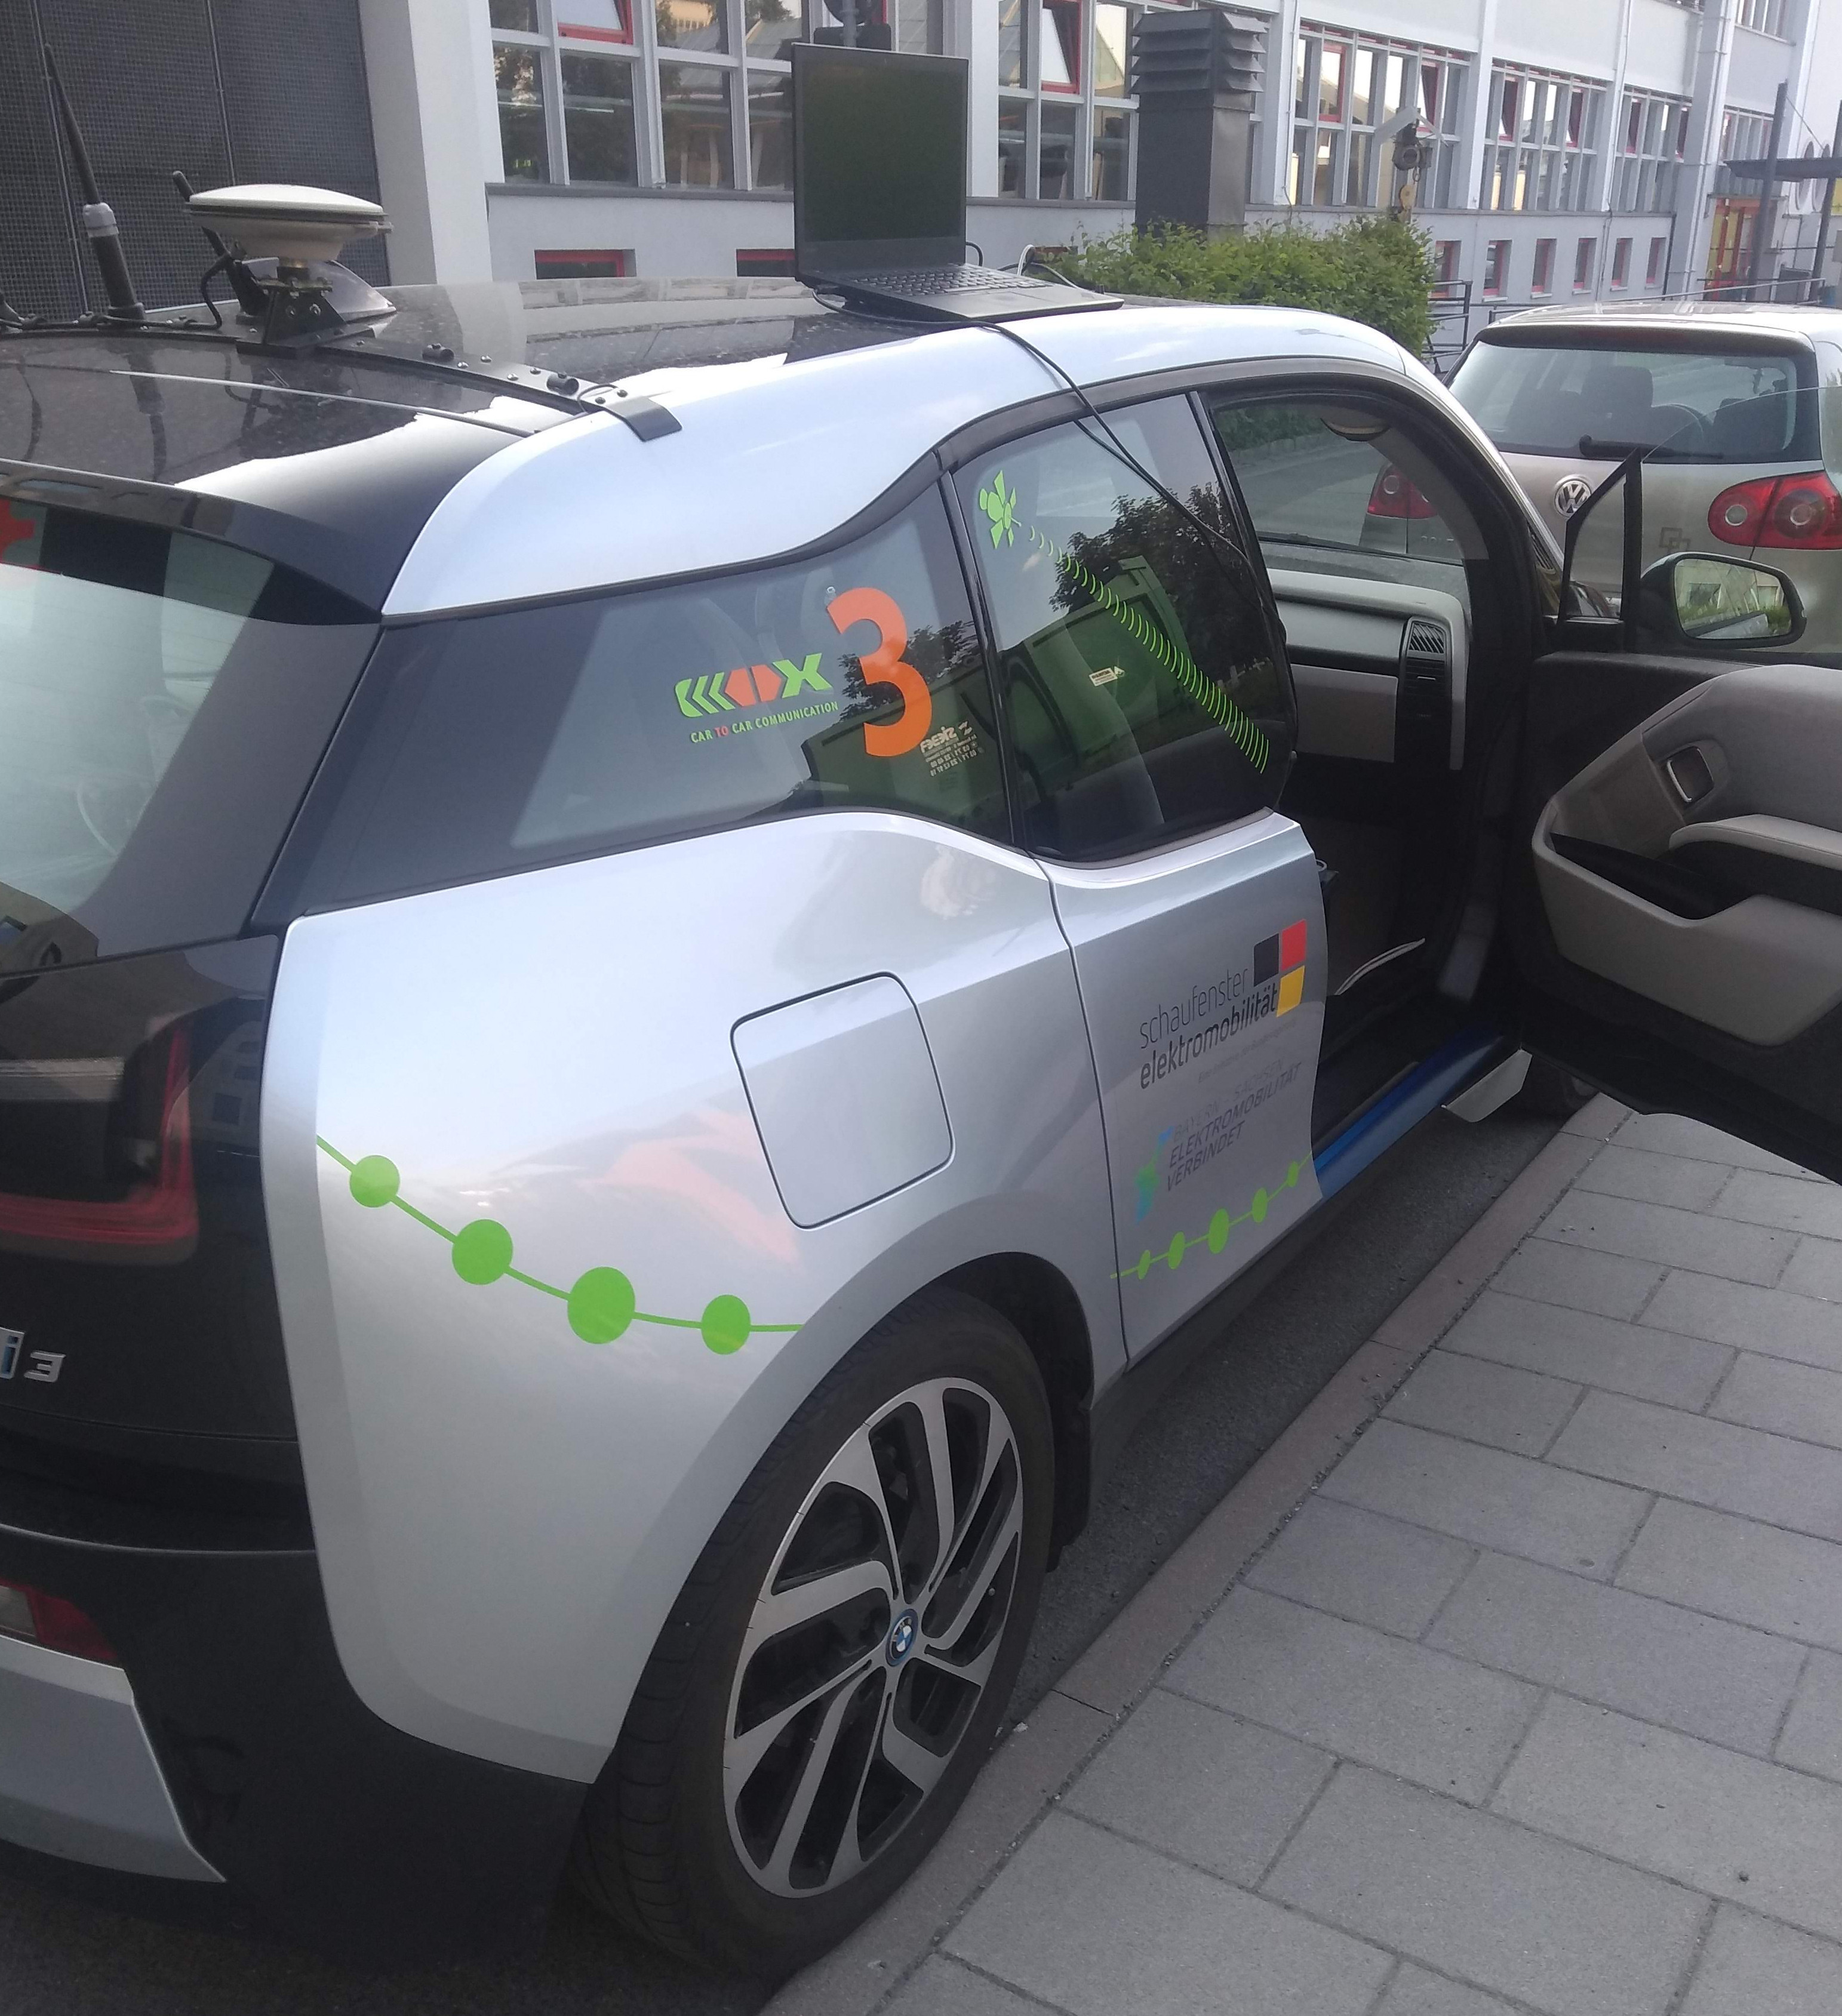
\includegraphics[width=0.5\textwidth]{Testvehicle}
      \label{fig:testVehicle}
  \end{figure}
   
  \section{Operation}
  This node provides positional estimates among other things as described earlier. It can be used with another node which provides a map service to plot the current location. This can be seen in the Fig. \ref{fig:gnsswithmap}
  
  \begin{figure}[h]
      \caption{Operation of the node visualized using a map}
      \centering
      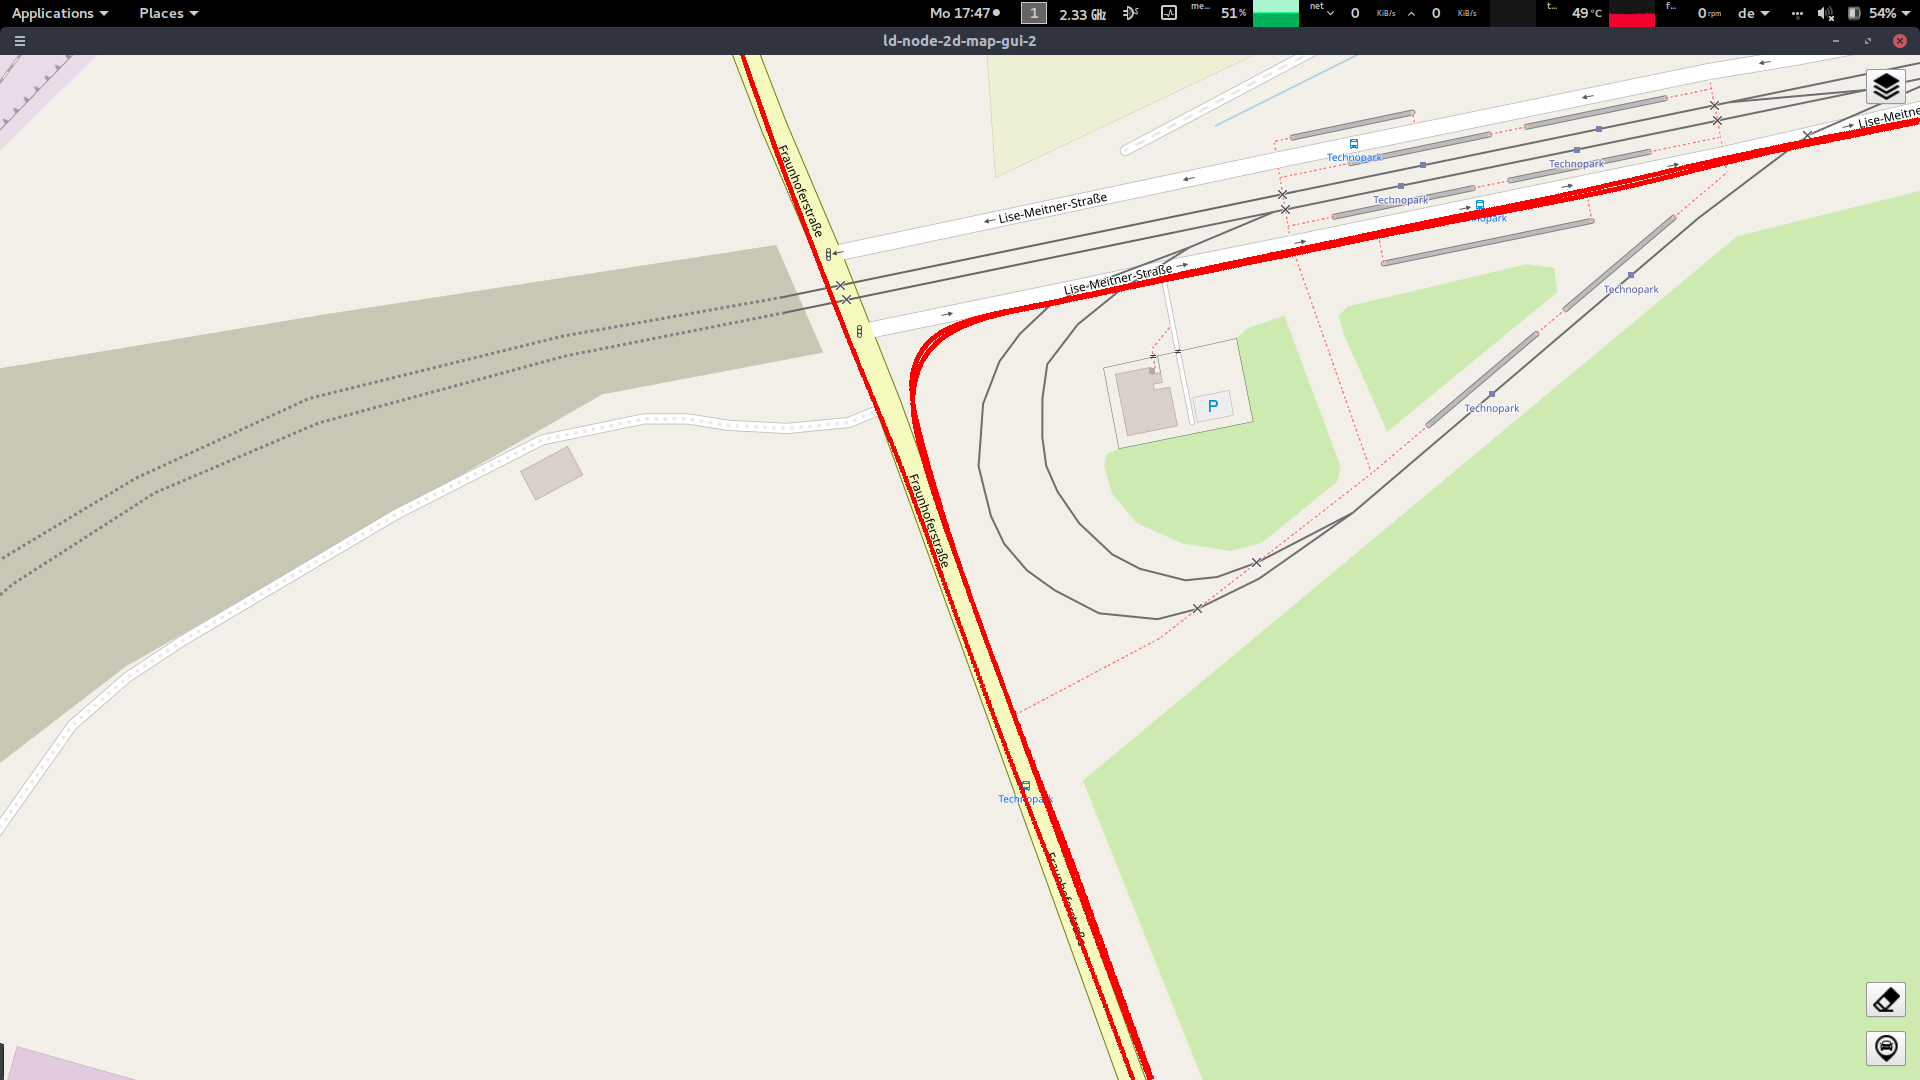
\includegraphics[width=0.7\textwidth]{gnsswithmap}
      \label{fig:gnsswithmap}
  \end{figure}

  \section{Analysis on the operation}
  
  While testing the operation of the node, it was observed that the signal from the satellites was not always reliable. occurrence of trees or tunnels for example would hamper the signal. This was of course expected. The Propak-V3 device however, also comes with an inertial measurement unit \cite{InertialmeasurementunitWikipedia-2020-02-02} which, according to design and specifications of the vendor, should compensate for the intermittent lack of satellite signals \cite{-2014-10-09}. However, it was observed that there were small but repeated durations when no position information was received from the receiver - satellite or IMU. It was important to understand exactly when this happened, i.e., I wanted to find out if there is a particular scenario which leads to this lack of signal. In addition, offsets were observed in the positional data received from the device. To do the analysis, I used the python package matplotlib \cite{MatplotlibPythonplottingMatplotlib313documentation-2020-02-09}. The data was recorded from the node itself in csv format. In figure \ref{fig:gnssavailability} you can see these messages availability is being plotted. This helped understand what was unexpected and when. BestPos is a message form the receiver which expresses the best guess of the receiver of the position \cite{-2014-10-09}. IMU messages also carry coordinates, but the data is from the IMU part of the device and not the satellite GPS positional data.
    
  \begin{figure}[h]
      \caption{Plotting the GNSS messages availability with time.}
      \centering
      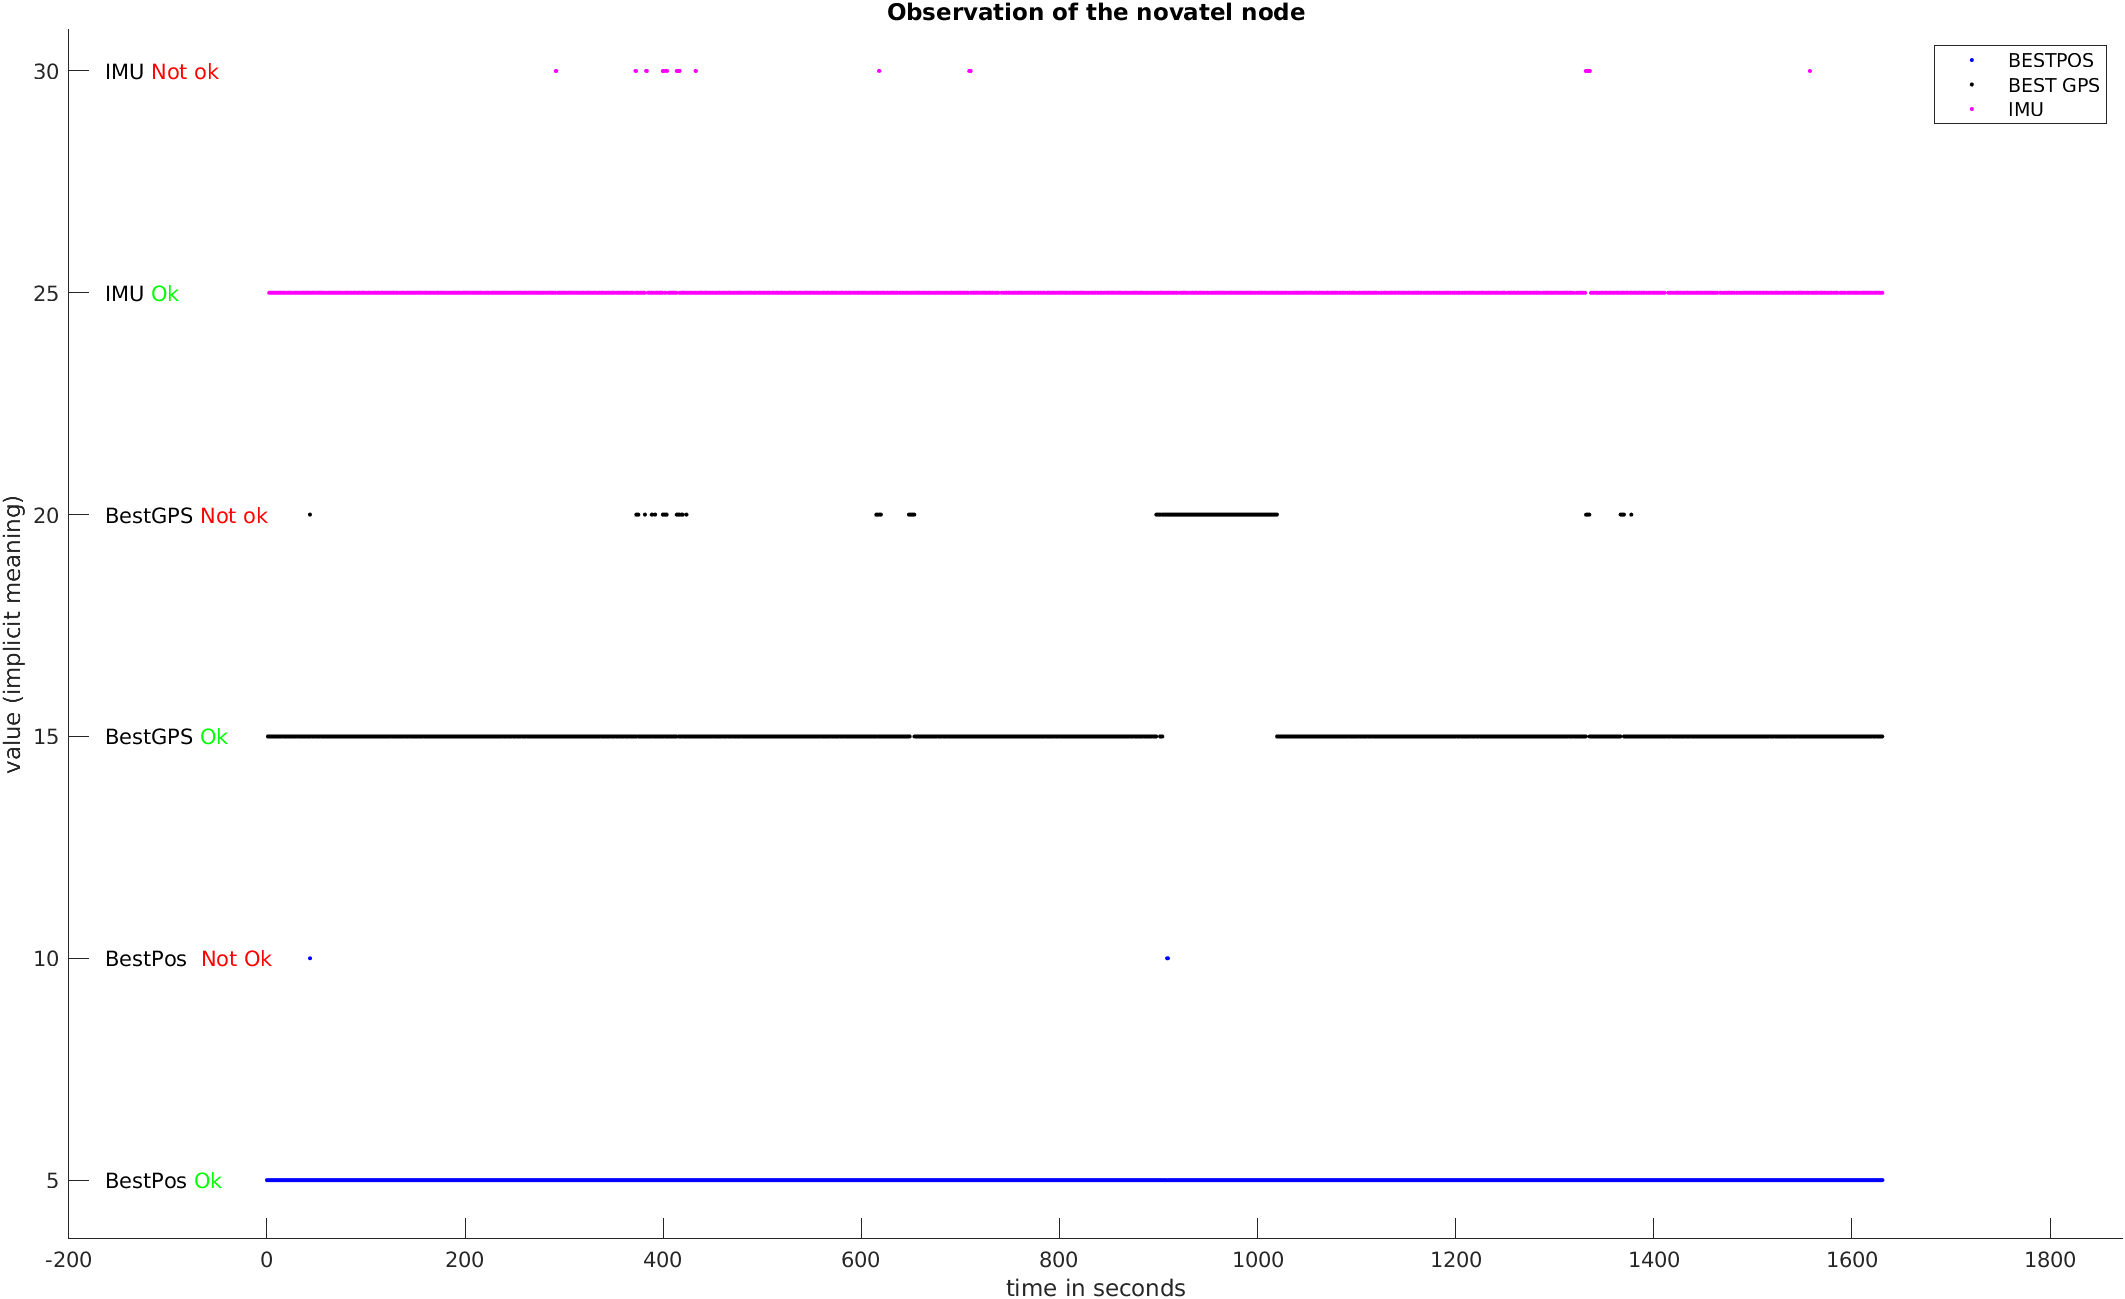
\includegraphics[width=1\textwidth]{TestDrive6_Visualized}
      \label{fig:gnssavailability}
  \end{figure}

  Further, to better understand what was happening, I took the GNSS receiver positional estimates and entered them into Google Maps service. The result of this can be seen in Fig. \ref{fig:plottingongmaps}
  
  In Fig. \ref{fig:plottingongmaps-offset} you will see a zoomed out section of the map. There is a ``jump" in the calculated position estimates which is clearly wrong. This was a concrete description of the problem. Why the device was generating such an offset is not known, but my speculation is that only the latitude was not getting updated correctly. The reason for this can be seen in Fig. \ref{fig:plottingongmaps-offset-corrected}. Note that a rotation of a few degrees leads to the positions aligning in a neat way.
  
 
  \begin{figure}[h]
      \caption{Adding NovAtel positional estimates to Google Maps.}
      \centering
      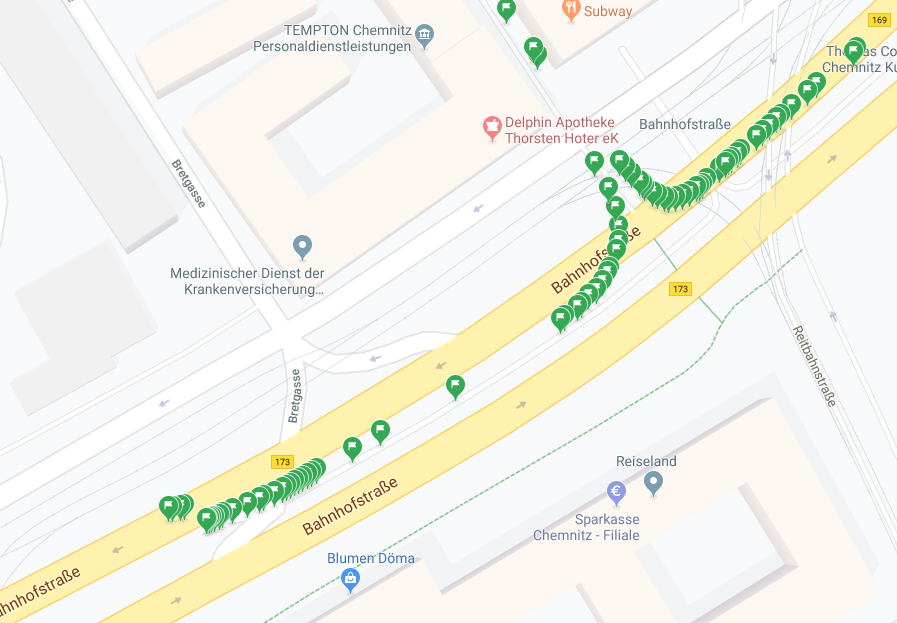
\includegraphics[width=1\textwidth]{plottingnovateldataongooglemap}
      \label{fig:plottingongmaps}
  \end{figure}

 \begin{figure}[h]
      \caption{Noticing the offsets in NovAtel positional estimates on Google Maps.}
      \centering
      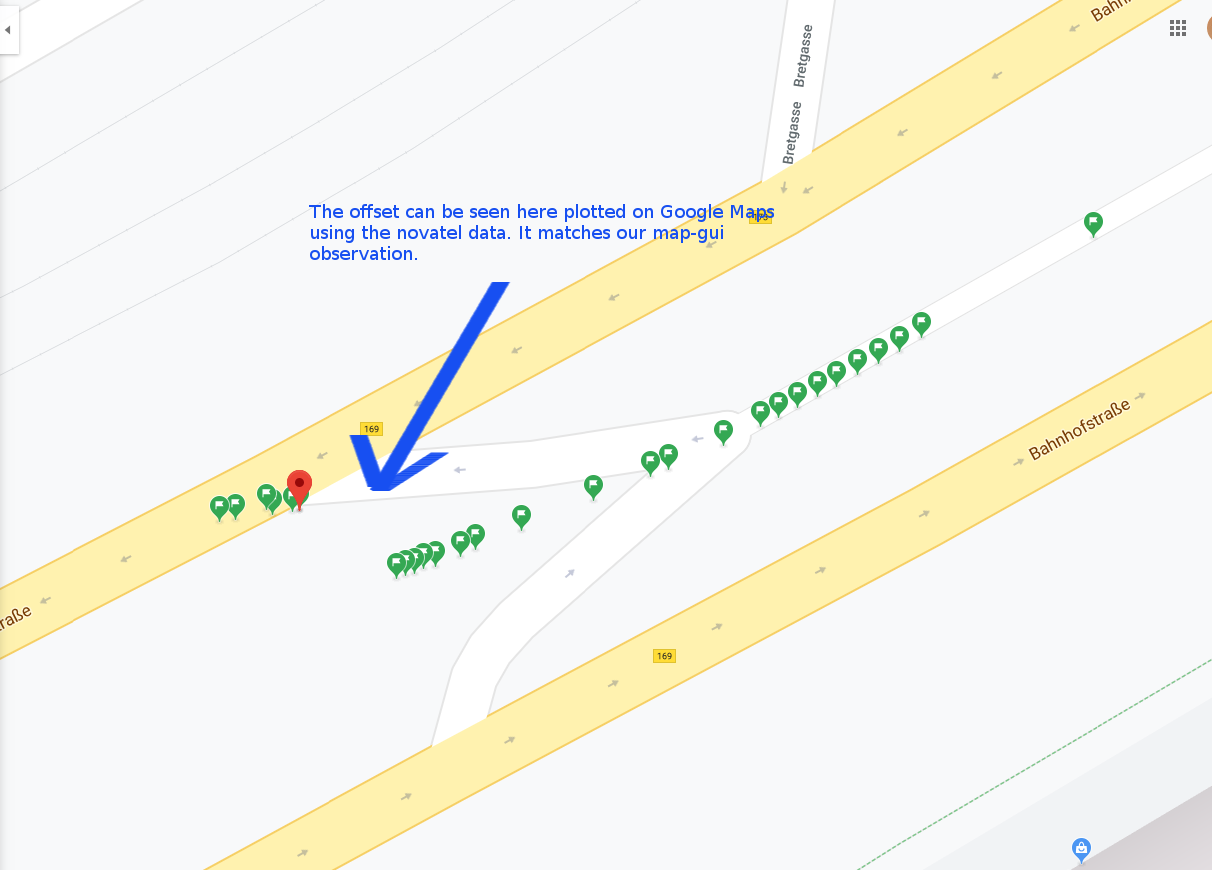
\includegraphics[width=1\textwidth]{offsetinmap}
      \label{fig:plottingongmaps-offset}
  \end{figure}

  \begin{figure}[h]
      \caption{Understanding the offset observed using Google Maps.}
      \centering
      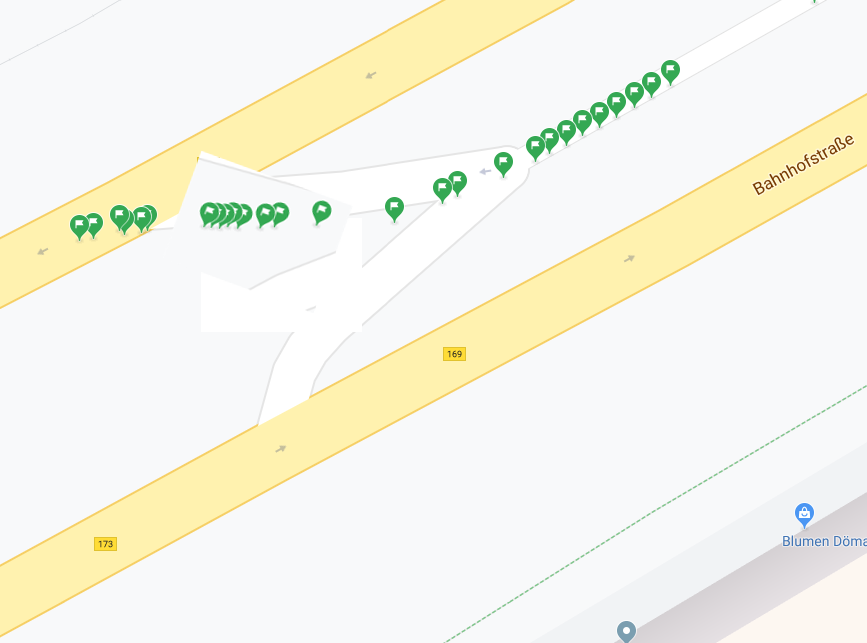
\includegraphics[width=1\textwidth]{offseterrorcorrected}
      \label{fig:plottingongmaps-offset-corrected}
  \end{figure}
            
  \newpage
  
  
  \chapter{Integration of machine vision cameras}

  \section{Allied Vision camera integration.}
  \subsection{Motivation and Context}
  This node, called \texttt{ld-node-camera-avt-2} \cite{NumericalAdvantageldnodecameraavt2ALink2nodetointerfacewithAlliedVisionMakoGmonochromemachinevisioncamera-2020-02-20} is designed to be an interface between Allied Vision GigE cameras \cite{MakoGDocumentationAlliedVision-2020-02-12} and the Link2 mesh. This node allows for configuration of the cameras and then the user is able to stream images captured from the camera (with desired frame-rate, image sizes, other camera settings) to the \textit{mesh}. Internally, this node uses the Vimba SDK provided by the manufacturer to interface with the cameras. Then it records images from the camera and writes the same thing on the mesh in \textit{Image} format which is internally defined.
  
  \subsection{Hardware set-up}
  The camera can be Powered over Ethernet or via a Hirose connector. I have used the PoE solution. 
  Fig. \ref{fig:hrdwr avt} shows what we want to achieve with the end result being that we have a network using the Ethernet on which both the camera and the computer running the node exist.
  We want to connect the camera to a computer which is running this node. For this to happen, it is needed to configure the IP and netmask for both camera and computer in such a way that they are on the same network. The camera was connected to a D-Link DGS-1008P Gigabit network switch \cite{DLinkDGS1008P8PortGigabitEthernetPoESwitchDLinkWorkscom-2020-02-17}. The switch in turn was connected to the computer via another Ethernet cable. Once you have this hardware set-up ready, now it is time to configure your IP and netmask on both camera and the computer with the aim of bringing them on the same network so that the camera is accessible to the computer being used to run the node. This same computer will also need to run Vimba SDK \cite{VimbaTheSDKforAlliedVisionCamerasAlliedVision-2020-02-17} on it. It might be necessary to increase the MTU \cite{MaximumtransmissionunitWikipedia-2020-02-10} for your Ethernet. On Linux it is done by \texttt{sudo ifconfig eth0 mtu <Desired\_Rate>}. It is important to check the data transmission rate of the camera, switch, computer network card. They should all match each other or there will be failures without error messages. 
 
 
  \begin{figure}[h]
      \caption{Hardware set up for GigE PoE Allied Vision camera.}
      \centering
      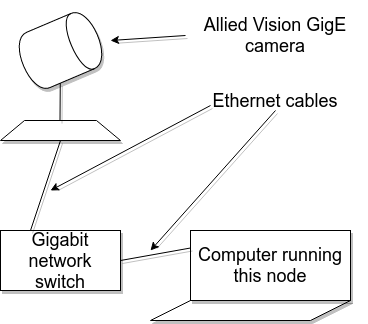
\includegraphics[width=0.7\textwidth]{avtcamera_hardware_set_up}
      \label{fig:hrdwr avt}
  \end{figure}
  
  \subsection{The Allied Vision Technologies Vimba SDK and how it was used}
  An overview of the Allied Vision Vimba SDK can be found in Fig. \ref{fig:vimba avt}. A detailed documentation of the Vimba SDK is available in \cite{VimbaCManualCPP-2020-02-17}.
  A simplified view of the C++ API in particular can be seen in Fig. \ref{fig:vimba avt_cpp_api} \cite{VimbaCManualCPP-2020-02-17}.
  
  \begin{figure}[h]
      \caption{Allied Vision Technologies Vimba SDK components overview \protect\cite{VimbaCManualCPP-2020-02-17}}
      \centering
      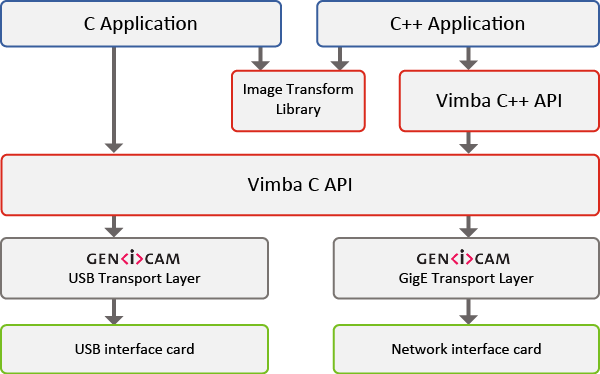
\includegraphics[width=0.7\textwidth]{Architecture-Linux}
      \label{fig:vimba avt}
  \end{figure}

  \vspace{0.2cm}
  
  \noindent I will now explain some crucial and technically interesting parts of the Vimba API.  
  
  \noindent Firstly, we need to use an instance of \texttt{VimbaSystem}. ``The entry point to Vimba C++ API is the VimbaSystem singleton. The VimbaSystem class allows both to control the API’s behavior and to query for interfaces and cameras" \cite{VimbaCManualCPP-2020-02-17}.

  \begin{lstlisting}[language=json,firstnumber=1]
  AVT::VmbAPI::VimbaSystem& m_vimbaSystem = 
  AVT::VmbAPI::VimbaSystem::GetInstance(); 
  AVT::VmbAPI::CameraPtr m_cameraPtr;
  \end{lstlisting}

  \noindent Next, I had to implement the interface \texttt{IFrameObserver} which contains the event handler function \texttt{FrameReceived}that gets called whenever a new frame is received \cite{VimbaCManualCPP-2020-02-17}.
  
  \begin{lstlisting}[language=json,firstnumber=1]
  class FrameObserver :   
              public AVT::VmbAPI::IFrameObserver 
  {
      public:
      FrameObserver(AVT::VmbAPI::CameraPtr pCamera, 
                    AVTCamDriver *pParent);
      
      /*!< Handler logic which runs when a frame is received. */
      void FrameReceived(const AVT::VmbAPI::FramePtr pFrame);  
      
      private:
      /*!< Pointer to the parent camdriver class*/
      AVTCamDriver* m_parent;  
  };   
  \end{lstlisting}
  
  \noindent To start capture of images, I had to do call the following function
  
  \begin{lstlisting}[language=json,firstnumber=1]
  m_camerPtr->StartContinuousImageAcquisition(NUM_FRAMES, 
                        AVT::VmbAPI::IFrameObserverPtr(
  new AVTCamDriver::FrameObserver(m_cameraPtr, this)));
  \end{lstlisting}
  
  \noindent And to stop acquisition I do the following (and then assuming I want to stop the node, call the shutdown function)
  
  \begin{lstlisting}[language=json,firstnumber=1]
  m_cameraPtr->StopContinuousImageAcquisition();
  m_vimbaSystem.Shutdown();
  \end{lstlisting}
  
  \noindent Inside my implementation of \textit{FrameReceived()} function, I write the captured image onto the \textit{mesh}. Note the use of OpenCV \cite{OpenCVAPIReferenceOpenCV24137documentation-2020-02-17} to convert the raw buffer of bytes to required image format. 
  
  \begin{lstlisting}[language=json,firstnumber=1]
  ...
  pFrame->GetBuffer(pBuffer);
  cv::Mat frame(imageSize, CV_8UC1, pBuffer);
  ...
  link_dev::ImageT currentImage 
  = link_dev::Interfaces::ImageFromOpenCV(frame, 
                link_dev::Format::Format_GRAY_U8);   
  
  m_parent->m_outputPin.push(currentImage, "AVTCamImage");
  ...
  \end{lstlisting}
    
  \subsection{Operation}
  When used with another \textit{node} called \texttt{ld-node-image-viewer-2}, the images captured by this node get displayed on a GUI. A sample can be seen in Fig. \ref{fig:avt_output}.
    
  \begin{figure}[h]
      \caption{AVT camera Node operation.}
      \centering
      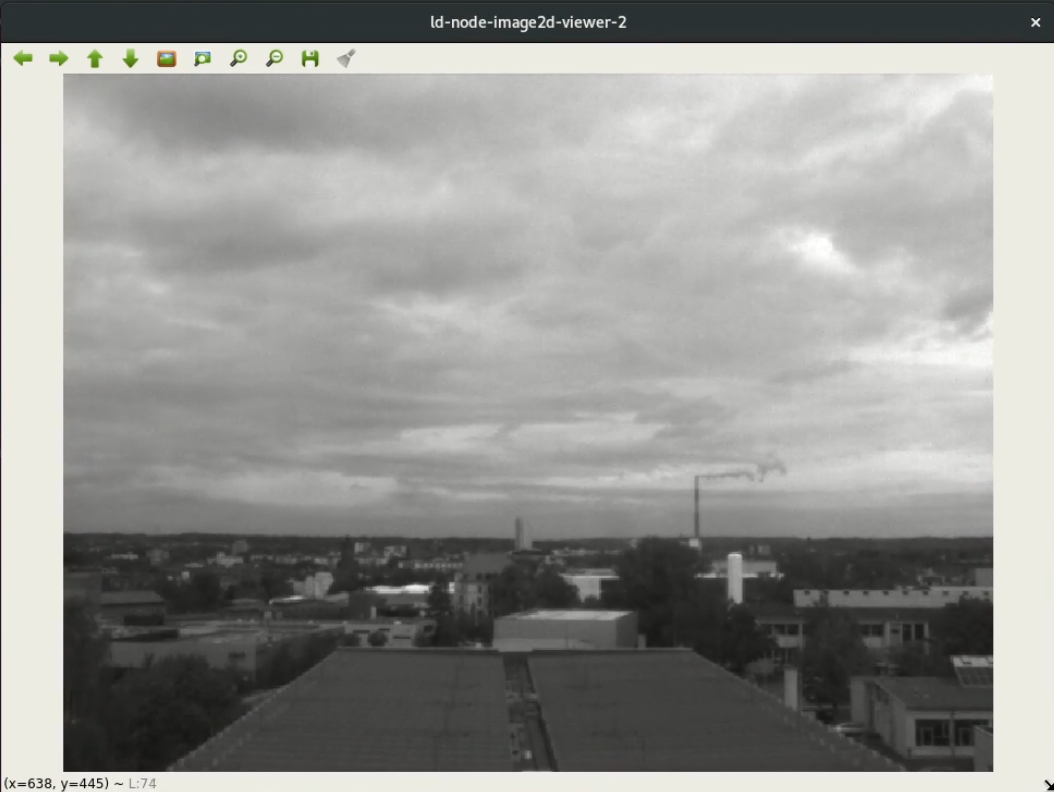
\includegraphics[width=0.9\textwidth]{avtcamoutput}
      \label{fig:avt_output}
  \end{figure}

  \begin{figure}[h]
     \caption{Vimba SDK simplified C++ API architecture \protect\cite{VimbaTheSDKforAlliedVisionCamerasAlliedVision-2020-02-17}.}
     \centering
     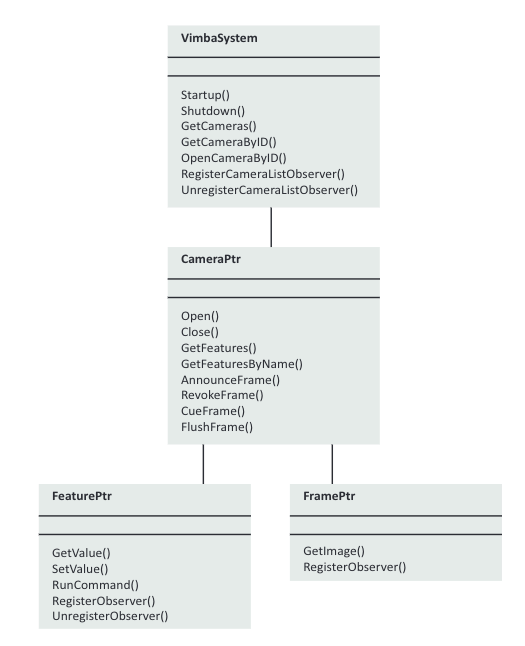
\includegraphics[width=0.9\textwidth]{vimba_cpp_simplified}
     \label{fig:vimba avt_cpp_api}
  \end{figure}
  
  
  \section{Basler camera integration}
  
  \subsection{Motivation and Context}
  The node \texttt{ld-node-camera-basler} \cite{NumericalAdvantageldnodecamerabaslerALink2nodetointerfaceaBasleraceseriesmachinevisioncamera-2020-02-20} is designed to be an interface between Basler GigE cameras \cite{BasleraceacA130075gcAreaScanCamera-2020-02-12} and the Link2 \textit{mesh} \cite{CorecomponentsDRAIVELinkDocumentation-2019-12-09}. This node allows for configuration of the cameras and then the user is able to stream images captured from the camera (with desired frame rate, image dimensions, other camera settings like auto exposure) to the mesh.
  Internally, this node uses the Pylon SDK provided by the manufacturer to interface with the cameras. Then it records images from the camera and writes the same thing on the mesh in \textit{Image} \cite{045ImageLinkDevelopersRFC-2020-01-16} format which is internally defined using FlatBuffers \cite{FlatBuffersFlatBuffers-2019-06-20} to store and represent images.
  
  \subsection{Hardware set-up}
  
  The camera used to develop this node was a BASLER acA1300-75gc \cite{BasleraceacA130075gcAreaScanCamera-2020-02-12}. The camera can be Powered over Ethernet or via a Hirose connector. In this particular setup I have used the PoE solution. To do this, a D-Link DGS-1008P Gigabit POE network switch \cite{DLinkDGS1008P8PortGigabitEthernetPoESwitchDLinkWorkscom-2020-02-17} was used. A library called Pylon \cite{pylonOpenSource-2020-02-14} is used internally to interface with the camera.
  Tools called \texttt{IpConfigurator} and \texttt{PylonViewer} are crucial in setting up the SDK and in troubleshooting and are part of the same Pylon open source library \cite{pylonOpenSource-2020-02-14}. 
  
  \subsection{The Pylon SDK and how it was used}
  I used the Pylon C++ API to interface with the Basler camera. An overview can be found in Fig. \ref{fig:pylon_arch}.
  
  \begin{figure}[h]
      \caption{Pylon C++ API overview \protect\cite{pylonOpenSource-2020-02-14}.}
      \centering
      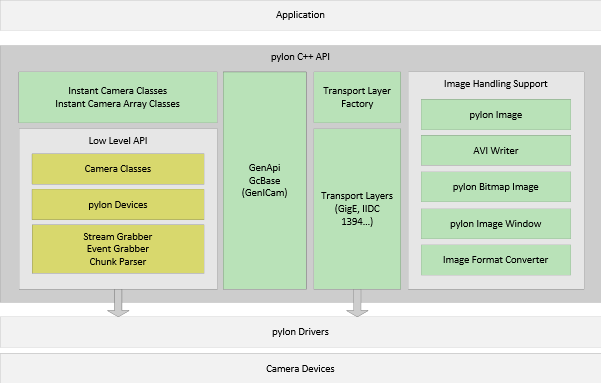
\includegraphics[width=1\textwidth]{pylon3_0_cpp_api}
      \label{fig:pylon_arch}
  \end{figure}

  \noindent Now I will present some of the important aspects of the Pylon SDK that I used to develop this node.
  
  \noindent I had to derive from a class called \texttt{CConfigurationEventHandler} which allows me to override a function called \texttt{OnOpened()} where I essentially out my handler code for when an image is ready to be grabbed. 
  
  \begin{lstlisting}[language=json,firstnumber=1]
  class BaslerCamDriver : 
     public Pylon::CConfigurationEventHandler
  {
    ...
    void OnOpened(Pylon::CInstantCamera& camera);
    ...
  \end{lstlisting}

  \noindent A camera object is created using an iterator which internally iterates over all connected cameras on the same network. In our case there is only camera. This is the central object which I will use to do all the other operations. 

  \begin{lstlisting}[language=json,firstnumber=1]
  ...
  Pylon::DeviceInfoList_t::const_iterator it;
  for(it = lstDevices.begin(); it != lstDevices.end(); 
      ++it )
  {
    Pylon::CBaslerGigEInstantCamera 
    camera(tlFactory.CreateDevice(*it));
    ...
  \end{lstlisting}
  
  After that operations to make particular settings on the camera and using it to capture images are possible. Pylon provides different ``grab strategies" \cite{pylonOpenSource-2020-02-14}, essentially balancing on demand use and availability and providing ability to control how resource intensive the application fetching images from the camera is. The strategy I am using is called ``OnByOne" \cite{pylonOpenSource-2020-02-14}.
  
  \begin{lstlisting}[language=json,firstnumber=1]
  camera.Open();
  camera.StartGrabbing(Pylon::GrabStrategy_OneByOne);   
  \end{lstlisting}
  
  The actual capture of images happens in a while loop like you see below. Note the use of \texttt{waitObjects} to ensure the thread with the while loop is not very CPU intensive. Essentially, the thread sleeps until there is image data ready to be grabbed. Without this mechanism there is a 4-fold increase in CPU usage. The \texttt{RetrieveResult()} function returns a pointer to the buffer inside the camera which contains the currently captured image. Note the use of OpenCV \cite{OpenCVAPIReferenceOpenCV24137documentation-2020-02-17} library to do necessary image data manipulations. Also note the usual Link2 API to push data onto the \texttt{Mesh} on line 25 of the following listing.
  
  \begin{lstlisting}[language=json,firstnumber=1]
  ...
  while(camera.IsGrabbing() && terminate == false)
  {
    if(!waitObjectsContainer.WaitForAny(0xFFFFFFFF, &index))
    {
      ...
      
      if(camera.RetrieveResult(0, ptrGrabResult, 
                       Pylon::TimeoutHandling_Return)) 
      {
        if(ptrGrabResult->GrabSucceeded())
        {
          if(outputFormat.compare("GRAY_U8") == 0)
          {
            uint8_t *pImageBuffer = 
            (uint8_t *)ptrGrabResult->GetBuffer();
            
            cv::Size imageSize(frameWidth, frameHeight);
            cv::Mat frame(imageSize, CV_8UC1, pImageBuffer);
            
            link_dev::ImageT currentImage =
            link_dev::Interfaces::ImageFromOpenCV(frame, 
                              link_dev::Format_GRAY_U8);   
            
            outputPin.push(currentImage, 
                           "BaslerCamImage");
            ...
       ...
    ...        
  \end{lstlisting}
    
  \subsection{Operation}
  
  When used with another \textit{node} called \texttt{ld-node-image-viewer-2} \cite{Image2DViewerLinkDevelopersRFC-2020-01-16}, the images captured by this node get displayed on a GUI. A sample can be seen in Fig. \ref{fig:baslerout}. Some manipulations on color hue and saturation were performed using the Pylon API but those changes were deemed unnecessary for the project. I analyzed the data rate generated by the camera at different settings (since different settings lead to different frame-rates and hence different requirements for bandwidth). I also created a way to measure the frames dropped during the capture process. This was useful to debug issues at run-time.  
  
  \begin{figure}[h]
      \caption{Basler camera node output with ld-node-imageviewer-2.}
      \centering
      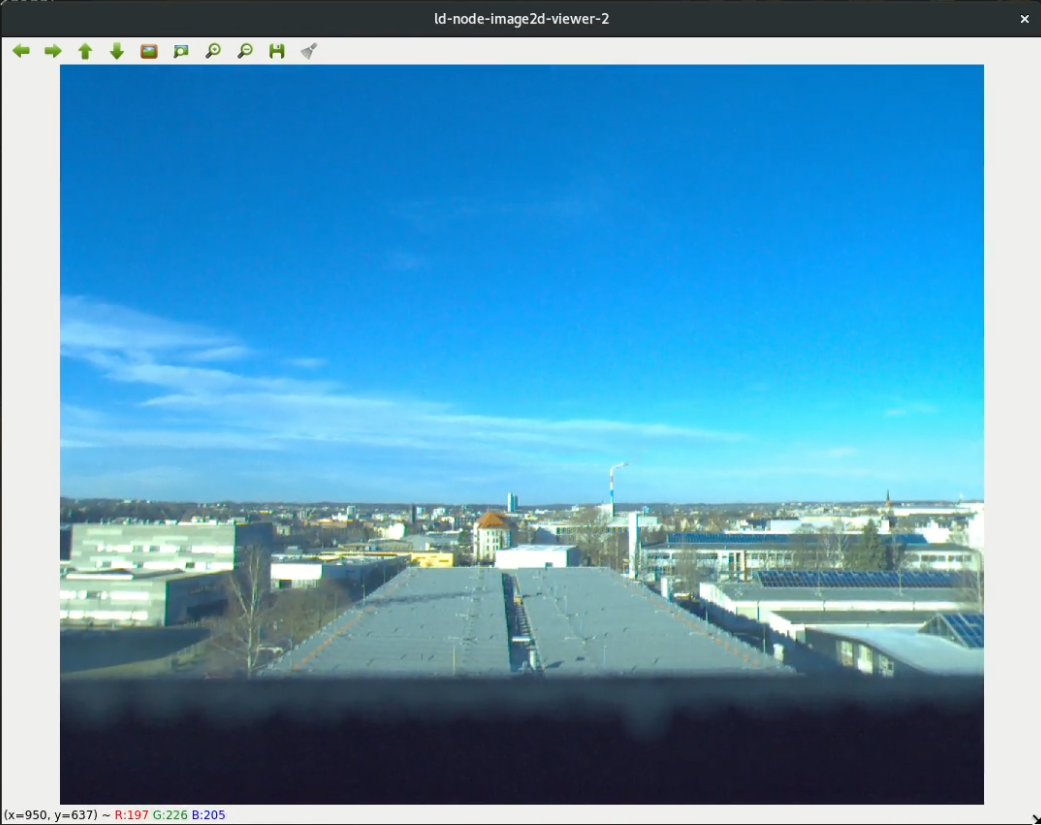
\includegraphics[width=1\textwidth]{basleroutput}
      \label{fig:baslerout}
  \end{figure}
  
  
  \newpage
  \chapter{Implementation of face detection and facial landmarks detection using the real-time Mesh}
  
  \section{Face Detection}
  \subsection{Motivation and Context}
  
  When supplied a video, this node, called \texttt{ld-node-face-detector-2}  \cite{NumericalAdvantageldnodefacedetector2ALink2nodetodetectfacesinastreamofvideo-2020-02-20} detects human faces in each individual frame of the video. This node runs in 2 modes depending upon the state of the \texttt{DebugMode} configuration parameter. In normal mode this node supplies the offer which contains the image in which faces are detected and the bounding box corresponding to each face and the number of faces detected. This will be clear from the next Data Profile section.
  From the RFC which this node implements: ``A bounding box MUST be described by the (u,v) coordinate of the top left corner and its width and height in pixels.". Note: A ``bounding box" describes a subset of the image for which it is defined. 
  Thus, in normal mode you get the original image back, with a set of set of 4 points which form rectangles in the image meant to denote faces that were found in the image.
  In debug mode, you get a video feed in real time (assuming a sufficiently fast computer. This is a computer with a NVIDIA Titan X GPU) with an overlay in black which shows you where the face(s) predictions were made on the frame.
  Internally this node uses \cite{dlibCLibrary-2020-02-12} to implement the max-margin object detection algorithm \cite{king2015max}. It uses a pre-trained model \cite{dlibCLibrarydnnmmodfacedetectionexcpp-2019-12-14} from dlib and makes heavy use of sample programs provided by dlib, viz. \cite{dlibCLibrarydnnmmodfacedetectionexcpp-2019-12-14}, \cite{dlibCLibraryfacedetectionexcpp-2019-12-14} and \cite{dlibCLibrarydnnintroduction2excpp-2019-12-14}.
  
  \subsection{Data Profile}
  
  New data formats had to be created using flatbuffers \cite{FlatBuffersFlatBuffers-2019-06-20} in order to be able to write data on the mesh. You can see them in the following listing.
  
  \begin{lstlisting}[language=json,firstnumber=1]
  table ImageWithBoundingBoxes
  {
    //Image in which the bounding boxes have been defined.
    imageWithFace : link_dev.Image;  
    
    //An array of bounding boxes. 
    boxes : [BoundingBox]; 
    
    //Number of bounding boxes.          
    numBoundingBoxes : int;
  }
  
  
  table BoundingBox
  {
    //top left corner of the bounding box.num_filters
    x_coordinate : int32; 
    
    //top left corner of the bounding box.
    y_coordinate : int32; 
    
    //width of the bounding box.
    width : int32;        
    
    //height of the bounding box.
    height : int32;
  }
  \end{lstlisting}
  
  \subsection{The dlib machine learning toolkit and how it is used here}
  Dlib contains a wide range of machine learning algorithms. All designed to be highly modular, quick to execute, and simple to use via a clean and modern C++ API. It is used in a wide range of applications including robotics, embedded devices, mobile phones, and large high performance computing environments \cite{dlib09}.
  
  \subsubsection{Subnet in dlib}
  From a practical standpoint, i.e. to be able to learn how to use the library, one of the first things one has to learn is the concept of a \texttt{subnet} and that of abstraction layers. It is very well described in \cite{dlibCLibrarylayersabstracth-2019-12-14}. A succinct explanation is in Fig. \ref{fig:subnet}.

  \begin{figure}[h]
      \caption{Meaning of subnet in dlib \protect\cite{dlibCLibrarydnnintroduction2excpp-2019-12-14}}
      \centering
      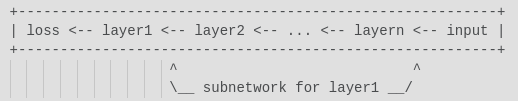
\includegraphics[width=1\textwidth]{subnet}
      \label{fig:subnet}
  \end{figure}

  \subsubsection{Building neural networks using templated aliases in dlib}
    
  Templated alias for a block which will take the sub-network passed to 
  it and pass it through a convolution layer with \texttt{num_filters} convolutions 
  with a 5x5 filter and 2x2 stride.
  
  
  \begin{lstlisting}[language=json,firstnumber=1]
  template <long num_filters, typename SUBNET> 
  using con5d = 
  dlib::con<num_filters, 5, 5, 2, 2, SUBNET>;
  \end{lstlisting}
  
  Templated alias for a block which will take the sub-network passed to 
  it and pass it through a convolution layer with \texttt{num_filters} convolutions 
  with a 5x5 filter and 1x1 stride.
  
  \begin{lstlisting}[language=json,firstnumber=1]
  template <long num_filters, typename SUBNET> using con5 = 
  dlib::con<num_filters, 5, 5, 1, 1, SUBNET>;
  \end{lstlisting}
  
  Templated alias for a block which will take the sub-network passed to it
  and apply 16 convolutions in the way as defined in the first block above
  which is then passed to an affine layer, the entire subnet following the 
  output of above is then subjected to another 32 convolutions of filter 
  5x5 and stride 2x2, followed by another affine layer and then a ReLU \cite{RectifierneuralnetworksWikipedia-2020-02-10} 
  followed by another 32 convolutions.  
  
  It applies a simple point-wise linear transformation to an input tensor.  
  You can think of it as having two parameter tensors, $A$ and $B$.  If the 
  input tensor is called $INPUT$ then the output of this layer is:
  $A*INPUT+B$
  where all operations are performed element wise and each sample in the
  $INPUT$ tensor is processed separately \cite{dlibCLibrarylayersabstracth-2019-12-14}.
  
  \begin{lstlisting}[language=json,firstnumber=1]
  template <typename SUBNET> using downsampler = 
  dlib::relu<dlib::affine<con5d<32, dlib::relu<dlib::affine<con5d<32, dlib::relu<dlib::affine<con5d<16, SUBNET>>>>>>>>>;
  \end{lstlisting}
 
  Templated alias for a block which will pass the sub-network passed to it
  through 45 convolutions of filter size 5x5 and stride 2x2 followed 
  by an affine layer followed by a ReLU layer.
  \begin{lstlisting}[language=json,firstnumber=1]
  template <typename SUBNET> using rcon5 = 
  dlib::relu<dlib::affine<con5<45, SUBNET>>>;
  \end{lstlisting}
  
  Broadly speaking, there are 3 parts to a neural network definition.  
  The loss layer, a bunch of computational layers, and then an input layer. 
  You can see these components in the network definition below.
  The loss layer used is max-margin object detection \cite{king2015max}. You can see that an
  image (type dlib rgb) down-sampled with a ration of 6 to 5 forms the input.  
  The middle layers define the computation the network will do to transform the
  input into whatever we want. Here we see 4 layers of the block defined just above 
  being used.
  \begin{lstlisting}[language=json,firstnumber=1]
  using neuralNetType = 
  dlib::loss_mmod<dlib::con<1, 9, 9, 1, 1, 
  rcon5<rcon5<rcon5<downsampler<
  dlib::input_rgb_image_pyramid<dlib::pyramid_down<6>>>>>>>>;
  \end{lstlisting}
  
  The above is the final neural network that is used. Note that this \textit{design} of neural network is taken from \cite{king2015max}.
  
  Next we convert our images from video input to dlib using the following call:
  \begin{lstlisting}[language=json,firstnumber=1]
  dlib::assign_image(dlibImage, dlib::cv_image<dlib::bgr_pixel>(currentFrame));
  \end{lstlisting}
  
  Now tell the face detector to give us a list of bounding boxes
  around all the faces it can find in the image.
  \begin{lstlisting}[language=json,firstnumber=1]
  std::vector<dlib::mmod_rect>  detFaces = m_neuralNet(dlibImage);
  \end{lstlisting}
  
  \subsection{Fetching data from a different node}
  Note that in this node we also have an \textit{Input pin}. That is how we get the images on which we run the algorithm described in the previous subsection. Following listing makes clear how that works.
  Note the callback \texttt{DetectFaces()} in which I put the code for handling a new incoming image frame.
  \begin{lstlisting}[language=json,firstnumber=1]
  m_inputPin.addOnDataCallback("l2demand:/videoinput_thruimages", 
  [&](const link_dev::ImageT& receivedImage) 
  {
      DetectFaces(link_dev::Interfaces::ImageToOpenCV(receivedImage));
  });
  \end{lstlisting}

  \subsection{Pushing the data on the mesh}
  
  For each face that is found in current frame, create a \texttt{BoundingBoxT} object and 
  add a pointer to this object to the vector of bounding boxes in the flatbuffer \cite{FlatBuffersFlatBuffers-2019-06-20}.

  \begin{lstlisting}[language=json,firstnumber=1]
  BoundingBoxT currentBB;
  currentBB.x_coordinate = face.rect.left();
  currentBB.y_coordinate = face.rect.top();
  currentBB.width = face.rect.right()-face.rect.left();
  currentBB.height = face.rect.bottom()-face.rect.top();
  
  imageAndBB.boxes.push_back(std::make_unique<BoundingBoxT>(currentBB));
  \end{lstlisting}
    
  \subsection{Operation}
  When used in Debug mode with \texttt{ld-node-imageviewer-2} \cite{Image2DViewerLinkDevelopersRFC-2020-01-16}, the output in Fig. \ref{fig:facedetectputput} is produced. Note the demarcation of face. The camera used in the operation was an \textit{Allied Vision Mako GigE camera} \cite{MakoGDocumentationAlliedVision-2020-02-12} using  \texttt{ld-node-camera-avt-2} \cite{NumericalAdvantageldnodecameraavt2ALink2nodetointerfacewithAlliedVisionMakoGmonochromemachinevisioncamera-2020-02-20} node.
  
  \begin{figure}[h]
      \caption{Debug Output from ld-node-facedetector-2}
      \centering
      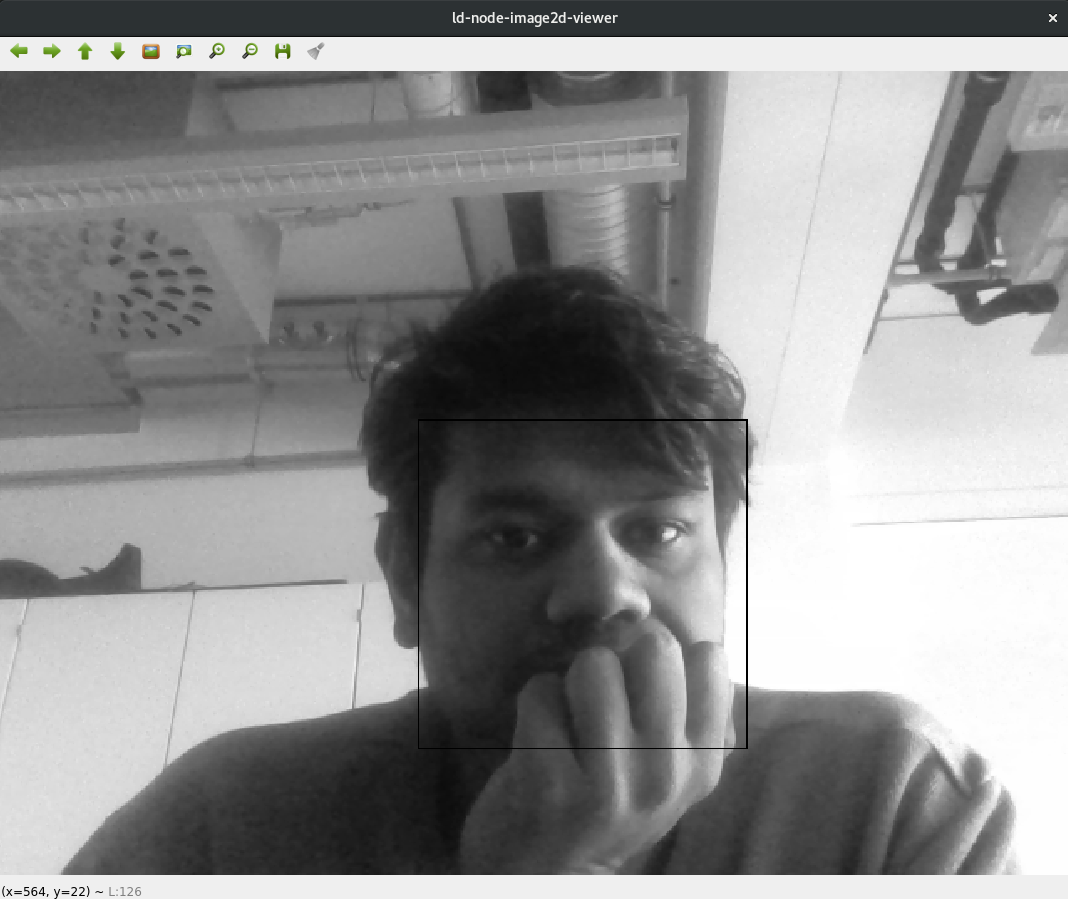
\includegraphics[width=1\textwidth]{facedetectionoutput}
      \label{fig:facedetectputput}
  \end{figure}
  
  \section{Facial Landmarks Detection}
  
  \subsection{Motivation and Context}
  
  The \textit{node} \texttt{ld-node-facial-landmark-detector-2} \cite{NumericalAdvantageldnodefaciallandmarkdetector2ALink2nodetodetectfacialfeatures-2020-02-20} uses TensorFlow library and pre-built models to detect 68 ``face key points" on the image of face supplied. This image of face is generated by \texttt{ld-node-face-detector-2} \cite{NumericalAdvantageldnodefacedetector2ALink2nodetodetectfacesinastreamofvideo-2020-02-20} as described in the previous section. Note that \texttt{ld-node-face-detector-2} writes output in the form of the below flatbuffer \cite{FlatBuffersFlatBuffers-2019-06-20} listing. 
  
  \begin{lstlisting}[language=json,firstnumber=1]
  //Contains an Image and one or more set(s) of 
  //co-ordinates that define a bounding box 
  //inside the image.
  
  table ImageWithBoundingBoxes
  {
    //Image in which the bounding boxes have been defined
    imageWithFace : link_dev.Image;  
    
    //An array of bounding boxes.
    boxes : [BoundingBox];       
  
    //Number of bounding boxes.
    numBoundingBoxes : int;          
  }
  \end{lstlisting}
  
  The video output from a camera can be used to supply an input stream of images and every frame of the video will be scanned for faces (by \texttt{ld-node-face-detector-2}) and subsequently facial landmarks can be also marked by this node in real time (assuming a processor and GPU fast enough to do so). The pre-built TensorFlow models used in this node are obtained from \cite{feng2018prn} and \cite{lighttransportprnetinferC11portofYadiraFsPRNetinferenceonly-2020-02-18}.
  
  \subsection{TensorFlow C++ API and how it is used here}
  
  One of the first things that is done is to load the pre-built graph \cite{ImportingaTensorFlowGraphDefbasedModelsintoTensorFlowjs-2020-01-09} and create a session \cite{tensorflowClientSessionClassReferenceTensorFlowCorev210-2020-02-14} with it. 
  
  \begin{lstlisting}[language=json,firstnumber=1]
  ...
  tensorflow::GraphDef graph_def;
  
  /*Read the protobuf graph supplied by user*/
  Status load_graph_status = 
  ReadBinaryProto(tensorflow::Env::Default(), 
                  graph_filename, &graph_def);
  ...
  
  /*Create a tensorflow::session to execute the above graph*/
  session.reset(tensorflow::NewSession(
  tensorflow::SessionOptions()));
  
  Status session_create_status = 
  session->Create(graph_def);
  ...
  
  \end{lstlisting}
  
  Later, when individual frames and the bounding boxes that represent faces in the image are processed one by one by the node, we create an input tensor using the bounding box from the input and then use a session to make the predictions on line 12 in the below listing.
  
  \begin{lstlisting}[language=json,firstnumber=1]
  ...
  cv::Mat norm_face;
  croppedFace.convertTo(norm_face, 
                   CV_32FC3, 1.0 / 255, 0);
  Tensor inpTensor(DT_FLOAT, 
          TensorShape({ 1,256,256,3 }));
  float * inpPt = inpTensor.flat<float>().data();
  cv::Mat inpImg(256, 256, CV_32FC3, inpPt);
  norm_face.convertTo(inpImg, CV_32FC3);
  ...
  
  Status run_status = session->Run({ { input_layer, 
                                  input_tensor } },
                                  { output_layer }, 
                                                {}, 
                                 &output_tensors);
  ...
  \end{lstlisting}
  
  \subsection{Fetching Images with Bounding Boxes from ld-node-face-detector-2 and publishing output}
  
  Note that we need \texttt{ImageWithBoundingBoxesT} in order to function. This \textit{subscription} is done in the following way -
  \begin{lstlisting}[language=json,firstnumber=1]
  m_inputPin.addOnDataCallback("l2demand:/image_with_bounding_boxes", 
  [&](const ImageWithBoundingBoxesT& imageWithBB)
  {
      HandleNewFrame(imageWithBB.imageWithFace, imageWithBB.boxes);
  });
  \end{lstlisting}
  
  Some image transformations are used after running the TensorFlow session to get the landmarks from the predicted output and these are published onto the mesh.
  
  \begin{lstlisting}[language=json,firstnumber=1]
   m_outputPin.push(
       link_dev::Interfaces::ImageFromOpenCV(
                      allFacesLandmarks,
      link_dev::Format::Format_GRAY_U8),
              "l2offer:/imagesWithLandmarks");

  \end{lstlisting}
  
  \subsection{Operation}
  
  I created a \textit{mesh} with the following \textit{nodes}  
  \begin{itemize}
     \item  \texttt{ld-node-image2d-viewer-2} \cite{Image2DViewerLinkDevelopersRFC-2020-01-16}
     \item  \texttt{ld-node-face-detector-2} \cite{NumericalAdvantageldnodefacedetector2ALink2nodetodetectfacesinastreamofvideo-2020-02-20}
     \item  \texttt{ld-node-webcam-2} \cite{WebcamLinkDevelopersRFC-2020-01-16}
     \item  \texttt{ld-node-facial-landmark-detector-2} \cite{NumericalAdvantageldnodefaciallandmarkdetector2ALink2nodetodetectfacialfeatures-2020-02-20}
  \end{itemize}
  
  \noindent This can be visualized with another node called \texttt{ld-node-mesh-viewer} in Fig. \ref{fig:mesh_landmark}. 

  \noindent The output of this node can also be visualized in debug output and this can be seen in Fig. \ref{fig:landmarkouput}
  
  \begin{figure}[h]
      \caption{Debug output from ld-node-facial-landmark-detector-2}
      \centering
      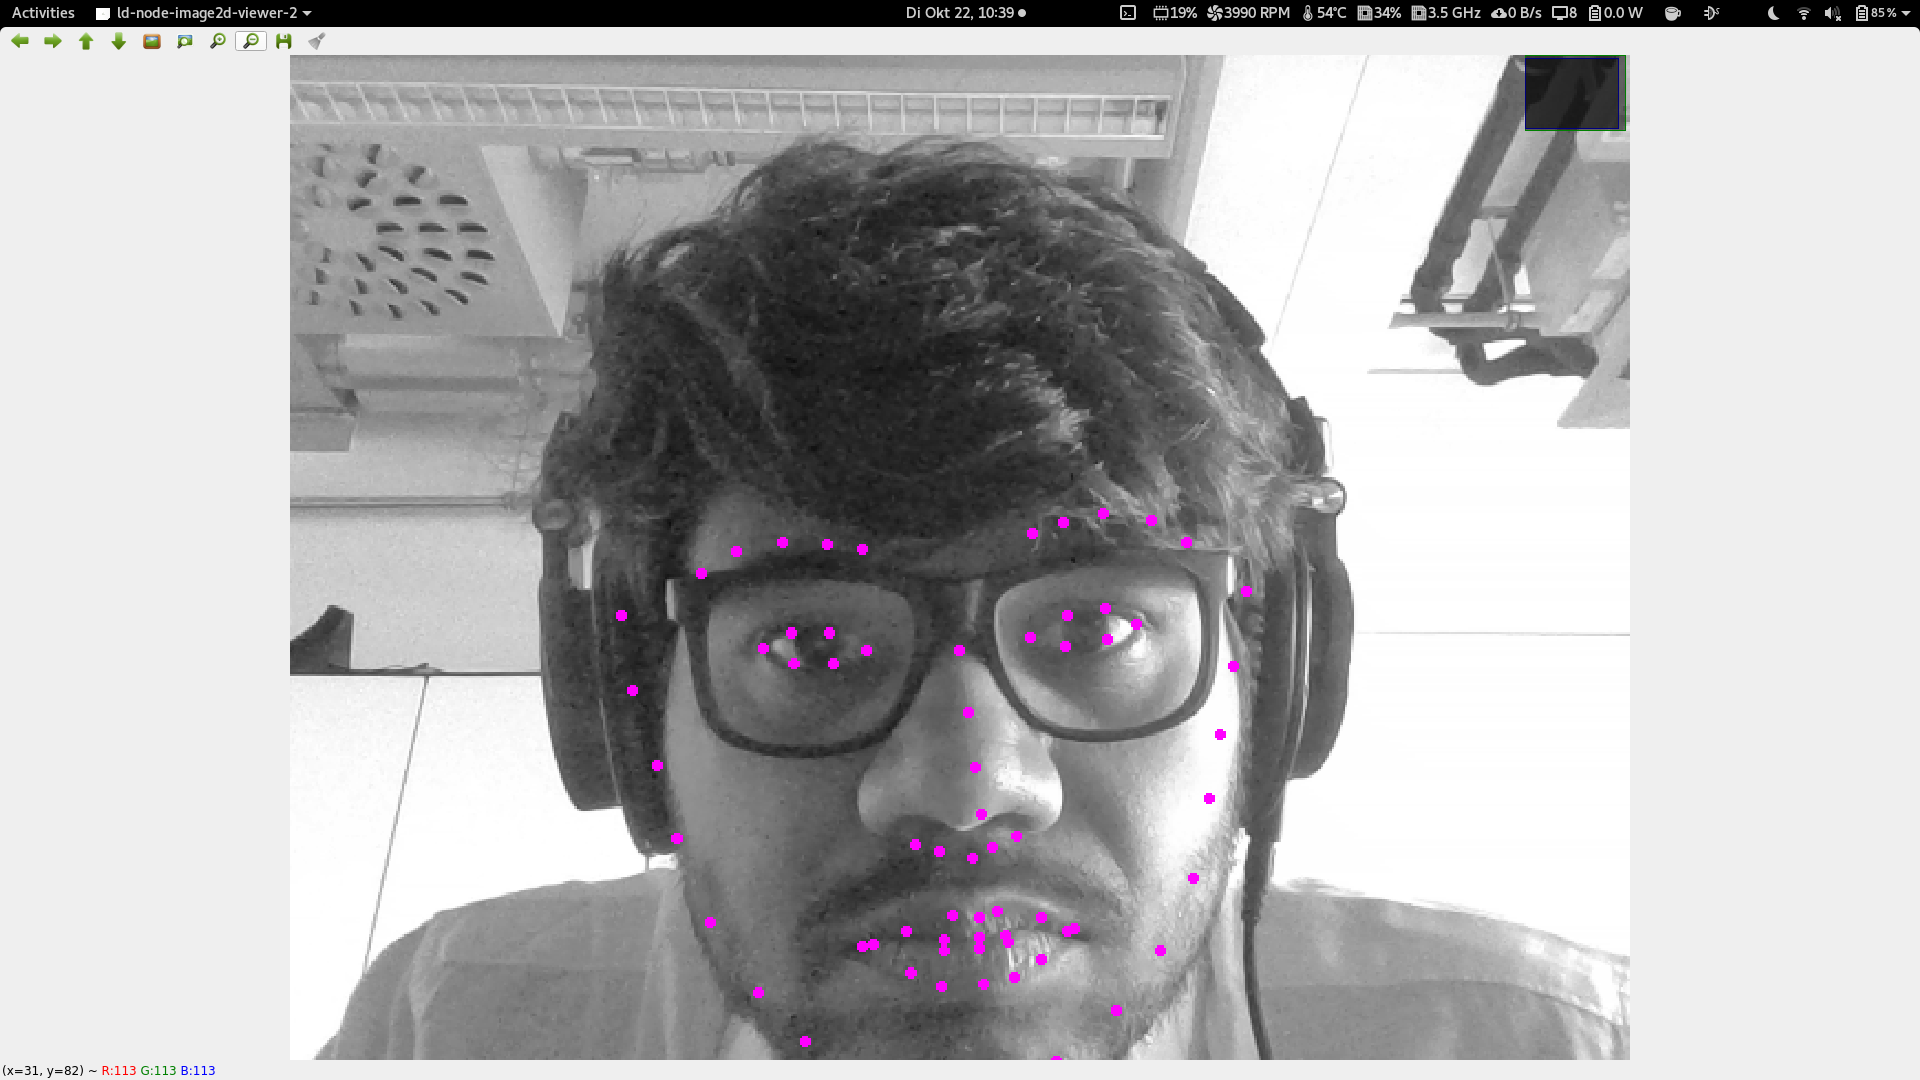
\includegraphics[width=1\textwidth]{faciallandmarkoutput}
      \label{fig:landmarkouput}
  \end{figure}

  \begin{figure}[h]
    \caption{View of the mesh for facial landmark detection}
    \centering
    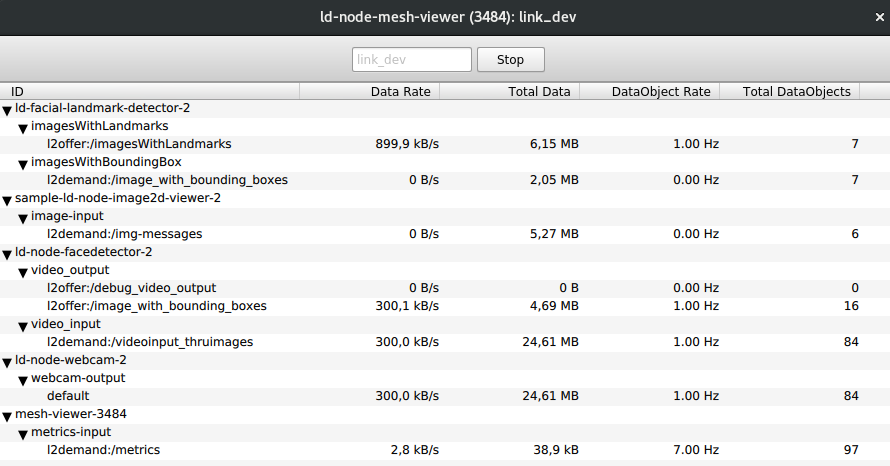
\includegraphics[width=1\textwidth]{mesh_viewer_on_sample_configuration}
    \label{fig:mesh_landmark}
  \end{figure}
   
  \newpage
  
  \chapter{Package configuration using conda}

  In order to maintain a repository of external libraries and packages, \texttt{conda} \cite{CondaCondadocumentation-2019-10-31} can be used. 
  Some important steps that I had to follow to do package configuration for the Pylon SDK \cite{pylonOpenSource-2020-02-14} with Gitlab CI pipeline \cite{CreatingandusingCICDpipelinesGitLab-2020-02-18} are described in this chapter. The end result was a \textit{package-config} \cite{cmakepackages7CMake3170rc1Documentation-2020-02-20} for the Basler Pylon SDK which can be deployed with conda \cite{CondaCondadocumentation-2019-10-31} and can be found in a Github repository \cite{NumericalAdvantagepylonsdkApackageconfigfortheopensourcePylonSDKformBaserAG-2020-02-20}.
  
  \section{The meta.yaml file}
  This file is necessary for things like specifying requirements for the build and host environments and specifying where exactly the package download is available from. 
  
  \begin{lstlisting}[language=json,firstnumber=1]
  ...
  package:
  name: "pylonsdk"
  version: "5.2.0"
  
  source:
  - url: https://hydrogen.draive.com/files/link_dev/pylon-5.2.0.13457-x86_64.tar.gz # [linux and x86_64]
  - url: https://hydrogen.draive.com/files/link_dev/pylon-5.2.0.13457-arm64.tar.gz # [linux and aarch64]
  - url: https://hydrogen.draive.com/files/link_dev/pylon-5-20191104T161031Z-001.zip # [win]
  
  build:
  number: {{ BUILD_VERSION }}
  
  requirements:
  build:
  - {{ compiler("c") }}
  - {{ compiler("cxx") }}
  
  ...
  
  \end{lstlisting} 
  
  \section{Telling conda how to create the necessary folder structure}
  
  This can be done like this - 
  
  \begin{lstlisting}[language=json,firstnumber=1]
  if [[ $target_platform == 'linux-aarch64' ]]; then 
  tar -xf pylonSDK-5.2.0.13457-arm64.tar.gz
  elif [[ $target_platform == 'linux-64' ]]; then 
  tar -xf pylonSDK-5.2.0.13457-x86_64.tar.gz
  fi
  
  PylonSDK_LIB_TARGET=$PREFIX/lib/
  PylonSDK_INCLUDE_TARGET=$PREFIX/include/
  
  mkdir -p $PylonSDK_LIB_TARGET
  cp -r pylon5/lib64/* $PylonSDK_LIB_TARGET
  
  
  mkdir -p $PylonSDK_INCLUDE_TARGET
  cp -r pylon5/include/* $PylonSDK_INCLUDE_TARGET
  
  cp $RECIPE_DIR/prefix/* $PREFIX -r
  
  echo "true";
  \end{lstlisting} 
  
  \section{Writing a CMake target import file for required configuration}
  
  Essentially we are letting \texttt{find\_package} \cite{findpackageCMake302Documentation-2020-02-20} find our manually created package. This consists of two major steps - creating imported targets \cite{ExportingandImportingTargetsWikiCMakeCommunityGitLab-2020-02-20} and setting property \cite{setpropertyCMake302Documentation-2020-02-20}. You can see this happening in the below listing.
   
  \begin{lstlisting}[language=json,firstnumber=1] 
  
  ...
  
  # Create imported targets 
  add_library(PylonGCBaseLibrary SHARED IMPORTED)
  set_target_properties(PylonGCBaseLibrary PROPERTIES INTERFACE_INCLUDE_DIRECTORIES 
  "${_IMPORT_PREFIX}/include")
  
  add_library(PylonGenAPILibrary SHARED IMPORTED)
  set_target_properties(PylonGenAPILibrary PROPERTIES INTERFACE_INCLUDE_DIRECTORIES
  "${_IMPORT_PREFIX}/include")
  
  add_library(PylonBaseLibrary SHARED IMPORTED)
  set_target_properties(PylonBaseLibrary PROPERTIES INTERFACE_INCLUDE_DIRECTORIES
  "${_IMPORT_PREFIX}/include")
  
  add_library(PylonUtilityLibrary SHARED IMPORTED)
  set_target_properties(PylonUtilityLibrary PROPERTIES INTERFACE_INCLUDE_DIRECTORIES 
  "${_IMPORT_PREFIX}/include")
  
  
  ...
  # Import targets for configuration "Release"
  set_property(TARGET PylonGenAPILibrary APPEND PROPERTY 
  IMPORTED_CONFIGURATIONS RELEASE)
  set_property(TARGET PylonGCBaseLibrary APPEND PROPERTY 
  IMPORTED_CONFIGURATIONS RELEASE)
  set_property(TARGET PylonUtilityLibrary APPEND PROPERTY 
  IMPORTED_CONFIGURATIONS RELEASE)
  set_property(TARGET PylonBaseLibrary APPEND PROPERTY 
  IMPORTED_CONFIGURATIONS RELEASE)
  
  ...
  
  set_target_properties(PylonGenAPILibrary PROPERTIES IMPORTED_LOCATION_RELEASE
  "${_IMPORT_PREFIX}/lib/libGenApi_gcc_v3_1_Basler_pylon.so")   
  
  set_target_properties(PylonUtilityLibrary PROPERTIES IMPORTED_LOCATION_RELEASE
  "${_IMPORT_PREFIX}/lib/libpylonutility-5.2.0.so")
  
  set_target_properties(PylonBaseLibrary PROPERTIES IMPORTED_LOCATION_RELEASE
  "${_IMPORT_PREFIX}/lib/libpylonbase-5.2.0.so")
  
  set_target_properties(PylonGCBaseLibrary PROPERTIES IMPORTED_LOCATION_RELEASE
  "${_IMPORT_PREFIX}/lib/libGCBase_gcc_v3_1_Basler_pylon.so")
  
  ...
  \end{lstlisting} 

  \section{Writing the CMakeLists file}
  Once the steps in the above sections are completed, the \texttt{CMakeLists.txt} from the below listing will work for our manually created package. 
  
  \begin{lstlisting}[language=json,firstnumber=1] 
  ...
  find_package(pylonsdk REQUIRED)
  add_executable(pylon_test main.cpp)
  target_include_directories(pylon_test PUBLIC)
  target_link_libraries(pylon_test 
                   PUBLIC PylonGenAPILibrary
                   PUBLIC PylonBaseLibrary 
                   PUBLIC PylonGCBaseLibrary
                   PUBLIC PylonUtilityLibrary)
  \end{lstlisting} 

  \section{Writing a CI Test for the newly created package}
  A small test was created like in the below listing
  
  \begin{lstlisting}[language=json,firstnumber=1] 
  #include <iostream>
  #include <GenICamVersion.h>
  #include <pylon/PylonIncludes.h>
  
  
  int main()
  {
      Pylon::PylonInitialize();
      Pylon::PylonTerminate();
      return 0;
  }
  \end{lstlisting} 
  
  
  The above test is executed by the CI pipeline using the code in the following listing
  
  \begin{lstlisting}[language=json,firstnumber=1] 
  echo "Run simple test program (makes initialize and terminate API calls)"
  
  mkdir -p pylon_test/build && cd pylon_test/build
  cmake -DCMAKE_CXX_COMPILER=$GXX -DCMAKE_CXX_FLAGS=$CXXFLAGS ..
  make -j$CPU_COUNT pylon_test
  ./pylon_test
  
  \end{lstlisting} 

  \newpage
  
  \chapter{Conclusion}
  
  A wide variety of problems which include autonomous driving are solved using a mix of different kinds of sensors like GNSS, camera, Radar, LiDAR. Independent components of a system might have the need for particular type of sensor data while there might be a lot more of sensor data being collected in the overall system. Different components might need the same sensor data, i.e. a many to one relationship. Most importantly, we are generally dealing with problems which need the data in real-time. This creates the need of a sensor fusion platform like Link2 \cite{ReactiveMeshforRealtimeDataProcessingDRAIVELinkDocumentation-2019-12-09}.
  
  Reverse engineering using simple tools like \cite{Aircrackng-2020-02-12} can reveal a lot about product design and even operation as can be seen from the work done for hacking the GoPro Hero7 \cite{GoProHERO7BlackInsanelysmooth4kVideo-2020-02-12} and its Smart Remote \cite{GoProSmartRemoteControl-2020-02-12} accessory in \cite{NumericalAdvantageGoProHackHackingtheWirelessUDPcommunicationbetweenGoProHero7andSmartRemotedevice-2020-02-20}.
  
  It is not enough to simply follow the API provided by the vendor of the sensor in order to guarantee performance. A wide variety of tests should be created to test the sensor in different conditions. Benchmark should be created for defining adequate performance and the sensor should be tested in all such circumstances. Software should assume failure can occur and should provide a way to register the failure for further analysis.
  
  Sensors like cameras have an extremely broad range of capabilities. Selecting the right model for the right job is often not trivial, especially when cost is accounted for. Different vendor API's will have different properties and behavior and relying too much on the "vendors way of thinking" is not a good idea. 
  
  Machine Learning is a fast evolving field with technologies changing fast. Learning to be an effective applications engineer in this field is an important skill to develop. This mainly consists of familiarizing oneself with different tool-kits and frameworks to do machine learning. Training models is a hard job. Not only does it require a lot of very specific technical and mathematical skills, but also considerable computing power resources and access to cutting edge and expensive hardware like Graphic Cards. However, by clever selection of models which other people have already trained, we can get a lot done in terms of proof of concept, selecting the right machine learning technique and experimentation. Such experimentation goes a long way in fulfilling scientific demands which are otherwise too resource consuming to be done. In order to keep up, a constant state of experimentation and an attitude of quick prototyping is necessary. This would usually mean keeping up with how people organize raw data in different machine learning frameworks and tool-kits like TensorFlow, PyTorch, dlib, many others and learning about novel machine learning models that are published and understanding how to use them for our own applications. 
  
  Effective documentation of software is necessary to provide a smooth transition from software proof of concepts to final delivery of software products. I achieved this from writing RFC's to simple README files for every software component developed. 
  
  Package management \cite{CondaCondadocumentation-2019-10-31} goes a long way to develop effective and hassle free open source software. Continuous Integration and Continuous Delivery using mature pipelines \cite{CreatingandusingCICDpipelinesGitLab-2020-02-18} offered by GitLab for example, are very effective tools to manage software repositories and keeping the product \textit{shippable} at all times.
  
  I also found that avoiding unnecessary jargon, keeping clarity of thought and process, understanding basic and essential building blocks of any system or framework, using uncomplicated language both in documentation and while writing code; are unparalleled tools to produce effective software systems. 
  
  \newpage
    
  \appendix
  
  \chapter{Guidelines for conducting effective test drives}
  
  \section{The guidelines}
  \normalsize I had to conduct a total of 11 test-drives when I was working on the GNSS receiver. I enumerated a set of points which are meant as guidelines for anyone who is going for a test-drive. These guidelines were added to the user-guide \cite{IntroductionStudentGuide-2020-01-20} and I am repeating them here:
  
  \begin{itemize}
  	
  	\item   Write down why you are going for this test drive. What do you aim to accomplish? What do others expect? Sure you have a good idea why, but have you confirmed with others interested in this test drive? Talk with them. Try to frame a simple single line ``purpose" and confirm this with others. This is the most important thing to consider. It may affect the way you conduct the test drive, the locations you choose to go, various settings, configurations.
  	
  	\item  Once you have enlisted the solid reason(s), motivation(s) for the test drive, think what data you would generate and in what format. Have a clear picture of what data you want to record and how you will do it. Do you need extra tools? Is your recording fully automatic or requires manual intervention? Do you have any concerns about your tools not working? Do you need to test them first before you start the actual test drive? Think about any likely but easily unforeseen situations. For example, if you are using some sort of map service and it is possible that you might not have Internet during the test drive, then you would probably want to cache the map before you start! Also, many times the data that you generate during your test drive is going to be volume intensive. So try to record data (for example your log files) in a way that it is easy to read and parse it using programming.
  		
  	\item Do you have any special requirements in the test drive? Should the car go through tunnels? Does the car need to be on a busy street or a highway? If there are such special requirements, make sure you talk about it with the person driving the car beforehand. Ideally, you should have a route prepared already.
  		
  	\item Might be beneficial to create small tables or text files in which you type in various kinds of details during the test drive. You should keep a ``diary style" or ``minutes of meeting" style record of the things that happen during the test drive. This could come in very handy.
  			
  	\item To sum it up shortly, be ready with a detailed ``test drive plan" and have someone look at it before the test drive. Communicate with your driver about your objectives from the test drive and try to gather as much information as possible and try to make it easier for you do so (better organization, automation, tools).  
    	
  \end{itemize}
  
  \section{Example of a test drive plan}	
    
  \begin{description}[labelindent=1cm]
      \item [Warm up and sanity test] Start node while car is stationary but out in the open. Test if the node works. 
      Cache the map.
      
      \item [Check operation of node without IMU] Start recorder. Start map-gui. Don't enable IMU. Test if node works. Check if logs are created properly. 
      Stop recorder. Save the recorded file. Stop map-gui.
      
      \item[Check operation of node with IMU] Start recorder. Start map-gui. Enable IMU. Test if node works. Check if logs are created properly.
      Stop recorder. Save the recorded file. Stop map-gui.
      
      \item[Check if ``status" is getting recorded when solution status is not good] Start recorder. Start map-gui. Enable IMU. Cover gnss receiver with hands. Test if node works. Check if logs are created properly. Stop recorder. Save the recorded file. Stop map-gui.
  \end{description}
   	
  \section{Example of a test drive log}
  
  \begin{description}[labelindent=1cm]
      \item [16:38]    Trees overhead
      
      \item [16:39]    A lot of IMU outage
      
      \item [16:39:48] Trees
      
      \item [16:41]    Small under-bridge
      
      \item [16:46:32] Big tunnel
      
      \item [16:48]    Possible offset or missing BESTPOS messages
      
      \item [16:51]    GPS and INS both failed - trees and bad roads
      
      \item [17:24:31] Trees
      
      \item [17:26:25] Tunnel (big)
      
      \item [17:28:30] Building and some trees
      
      \item [17:33]    Small under-bridge   
  \end{description}
        
  \newpage
  
  \chapter{Guidelines for using media in software documentation}
  
  \normalsize I wrote a few guidelines for using media like pictures, GIF's, video in software documentation which was later included in the user-guide \cite{IntroductionStudentGuide-2020-01-20}. 
  Here are the points I came up with: 

  \begin{itemize}
  	\item Media is a great way to add substantial value to your documentation, making it very easy to provide instant context to what problem your software solves, or how. A short demonstration can also be generally included in the README via pictures, videos, GIF's. Below are some guidelines which can help you to add better value minus the clutter.
  	
  	\item Your media should be on point. It should not contain anything else that may confuse the reader. For example, if you want to show a camera, then having a laptop in the same picture as the camera may lead the reader to believe that perhaps the laptop is also needed for the operation of the camera.
  	
  	\item Environment of the media should be consistent with the purpose of the project. For example, if your project is about using computer vision on vehicles, then your demonstration should use vehicles (and not apples for example).
  	
  	\item When showing a demonstration, it would be nice to have a textual prompt somewhere on the screen which ``narrates" the demonstration to the reader. Note that GIF's don't have sound.
  	
  	\item Sometimes you may be tempted to use a picture where a simple diagram might suffice. Don't forget to use the ``simplest way" first. Don't use a picture (or other media) where a diagram would be enough.
  	
  	\item Always aim for easier, faster and better understanding of the reader when you embed media to your software documentation.
  	
  	\item The media that you use, should in no way divulge any personal information or any identification of instruments, tools, infrastructure in any way. Do not overlook privacy concerns of not just yourself, but others as well.
  \end{itemize}

  \newpage
  
  \chapter{Git forking workflow}
  
  \normalsize Throughout my tenure of internship, I was required to follow the ``forking model" git workflow to organize my source code and for activities like continuous integration, code review, collaboration with the rest of the team. Detailed information on this subject can be found at \cite{UsingtheForkandBranchGitWorkflowScottsWeblogTheweblogofanITprofocusingoncloudcomputingKubernetesLinuxcontainersandnetworking-2020-01-01} and \cite{ForkingWorkflowAtlassianGitTutorial-2020-02-12}. 
	
  \vspace{0.2cm}	
  \noindent In short, the git forking workflow is to be followed through the following steps:
  
  \begin{itemize}
  	\item	Fork a Git repository.
  	\item	Clone the forked repository to your local system.
  	\item	Add a Git remote for the original repository.
  	\item	Create a feature branch in which to place your changes.
  	\item	Make your changes to the new branch.
  	\item	Commit the changes to the branch.
  	\item	Push the branch to Git.
  	\item	Open a pull request from the new branch to the original repo.
  	\item	Clean up after your pull request is merged.
  \end{itemize}

  \normalsize \noindent I found this style of managing source code change, versioning and collaboration to be effective for the following reasons:
  
  \begin{itemize}
  	\item	It uses git! Git is very popular and implicitly supports the decentralized way of building software.
  	\item	The model is rather simple.
  	\item	It is easy to get used to the model and not make a lot of mistakes. 
  	\item   It establishes a strict contract for a developer in terms of making contributions.
  \end{itemize}  
    
  \printbibliography[heading = bibintoc]

\end{document}